\chapter{Implementation}\label{Chapter:implementation}
This chapter presents the implementation of the \textit{Decomposition} project, which serves as a TNL-compatible framework for housing the CMPP and ICMPP algorithms described in Sections~\ref{Subsection:theory->ICMPP->LUP->CMPP} and \ref{Subsection:theory->ICMPP->LUP->ICMPP}, respectively.
In addition to these algorithms, a set of triangular solvers has been implemented to offer a comprehensive solution for solving systems of equations.

First, the 3rd party libraries used in the project will be presented.
Then, the project itself will be detailed.
Finally, the last section presents the integration of the Decomposition project into a library that aims to provide a solver of linear equations for systems originating from finite element computations.

\section{Libraries Used}\label{Section:implementation->libraries-used}
This section aims to introduce the two main libraries used in the \textit{Decomposition} project.
The first, \textit{Template Numerical Library (TNL)}\footnote{TNL website URL: \url{https://tnl-project.org}}, provides this project with data structures and parallel functionalities.
The second, \textit{CUDA Libraries} (\textit{cuSOLVER}\footnote{cuSOLVER website URL: \url{https://developer.nvidia.com/cusolver}}, \textit{cuBLAS}\footnote{cuBLAS website URL: \url{https://developer.nvidia.com/cublas}}), provides state-of-the-art decompositions and linear system solvers.

\subsection{Template Numerical Library (TNL)}\label{Subsection:implementation->libraries-used->TNL}
The Template Numerical Library (TNL) \cite{Oberhuber2021, Klinkovsky2022} is an open-source and collaborative project licensed under the MIT license.
According to the core team behind the project, TNL aims to be the C++ Standard Template Library (STL) for HPC \cite{prXEEmGjoxB89XBn}.
In practice, this means facilitating a base for the development of, for example, efficient numerical solvers and other HPC algorithms.
Similarly to STL, TNL is implemented in C++ and uses up-to-date programming paradigms to provide a user-friendly interface.
Additionally - as the name suggests - TNL utilizes the advantages provided by C++ templates such as minimal overhead runtime and broad compatibility of functionalities.
In terms of HPC, TNL provides a unified interface for managing multicore CPUs, GPUs, and distributed systems.

While TNL provides a wide range of data structures and functionalities, this section will only briefly present those utilized in the \textit{Decomposition} project.
First, a selection of data structures will be introduced followed by parallel functionalities.
See \citetitle{ixA8ZYptYohwlgwt} \cite{ixA8ZYptYohwlgwt} for examples and tutorials concerning the presented content.

\subsubsection{Data Structures}

\paragraph{Array} One of the most basic data structures is the \code{TNL::Containers::Array} class or \code{Array} for short \cite{ixA8ZYptYohwlgwt}.
An array type is declared using the following template parameters:

\begin{tight_itemize}
	\item \code{Value} - The array data type, e.g., \code{double}.
	\item \code{Device} - The device where an array operation is to be performed - either on the CPU or on the GPU, denoted using \code{TNL::Devices::Host} or \code{TNL::Devices::Cuda}, respectively.
	\item \code{Index} - The indexing data type, e.g., \code{int}.
	\item \code{Allocator} - The allocator type used for the allocation and deallocation of data.
This parameter dictates the memory space the data is allocated in, e.g., on the host (CPU memory space), or the device (CUDA memory space).
By default, the allocator corresponding to \code{Device} is set.
\end{tight_itemize}

At its core, \code{Array} contains a pointer to the data and the size of the array.
Additionally, methods providing different functionalities are present, for example, \code{resize()} or \code{forAllElements()}, where the latter executes a given lambda expression\footnote{C++ lambda expressions on cppreference: \url{https://en.cppreference.com/w/cpp/language/lambda}} for each element of the array; the lambda is executed by the same device whose memory space contains the data.
Note that while all methods can be executed on the host (CPU), only those prefixed with \code{\_\_cuda\_callable\_\_} can be executed on the device (Nvidia GPU).
The \code{\_\_cuda\_callable\_\_} macro is defined as \code{\_\_device\_\_ \_\_host\_\_}, where \code{\_\_device\_\_} indicates that the function can only be called from and executed on the device, and \code{\_\_host\_\_} indicates that the function can only be called from and executed by the host.

\paragraph{Vector} Extending \code{Array} is the \code{TNL::Containers::Vector} class \cite{ixA8ZYptYohwlgwt}.
Its template parameters are identical to that of \code{Array} except for changes in nomenclature.
While its parent class possesses functionalities largely centered around memory management, \code{Vector} adds basic vector operations such as addition, subtraction, scalar multiplication, etc.

\paragraph{Dense Matrix} The data structure implementing a dense matrix, i.e., a matrix storing all its values (zeros and nonzeros inclusive), is the \code{TNL::Matrices::DenseMatrix} class \cite{ixA8ZYptYohwlgwt}.
The class type is declared using the following template parameters:

\begin{tight_itemize}
	\item \code{Real} - The type of the matrix's elements, e.g., \code{double}.
	\item \code{Device} - The device where the matrix is allocated.
It can be either on the CPU or on the GPU denoted using \code{TNL::Devices::Host} or \code{TNL::Devices::Cuda}, respectively.
	\item \code{Index} - The indexing type of the matrix's elements, e.g., \code{int}.
	\item \code{Organization} - The ordering of matrix elements in the matrix's data vector.
It can be either row-major or column-major order, denoted by \code{RowMajorOrder} or \code{ColumnMajorOrder}, respectively, found in the \code{TNL::Algorithms::Segments::ElementsOrganization} namespace.
	\item \code{RealAllocator} - The allocator for the matrix's elements.
\end{tight_itemize}

Analogous to \code{Vector}, \code{DenseMatrix} contains a variety of functionalities ranging from different constructors and data accessors to matrix operations and per-element methods.

In this project, an often-used method is the data-accessing operator: \code{operator( row, col )}.
This operator returns a reference to an element at a given row and column.
While this access is fast, it can only be used to access data from the same device whose memory space contains the data as it is prefixed with \code{\_\_cuda\_callable\_\_}.
For cross-device data access, either \code{setElement( row, col, value )} or \code{getElement( row, col )} can be used.
Notwithstanding, the use of \code{setElement} and \code{getElement} is discouraged as copying a single element between devices is synonymous with low performance.
Note that \code{getElement()} returns the value of the element.

The \code{DenseMatrix} data structure was chosen to represent the matrices in the implementation presented earlier as the focus of this project is the development of a dense decomposition algorithm.

\paragraph{View} To comfortably use the aforementioned data structures in CUDA kernels, TNL provides an encapsulation mechanism without ownership in the form of \textit{views}.
For example, the \code{Array} class contains a view referred to as \code{ArrayView}.
It can be assimilated to a pointer to an \code{Array} instance that retains only methods of \code{Array} that do not manage memory.
Specifically, the \code{ArrayView} of an \code{Array} instance is bound to the \code{Array} instance's data via its data pointer, i.e., the data can be read and overwritten using the view but the array cannot be resized.
Note that the destruction of an \code{ArrayView} instance does not affect the \code{Array} instance.
Another important characteristic of \code{ArrayView} is that, unlike \code{Array}, its copy-constructor creates a shallow copy, i.e., only the pointer and size are changed.
This allows for array views to be both passed by value to CUDA kernels and captured by value in lambda functions (including lambda functions executed on the device).
In contrast, the overloaded operator \code{operator=} of both \code{Array} and \code{ArraView} performs a deep copy of the data.

\subsubsection{Parallel Functionalities}\label{Subsection:implementation->libraries-used->TNL->parallel-functionalities}

\paragraph{Parallel For Loop} Parallelization of a for loop performing independent tasks in CUDA is a simple task.
However, for user comfort, TNL provides a parallel for-loop implementation: \code{TNL::Algorithms::parellelFor( begin, end, f )}, where \code{begin} and \code{end} specify the boundary indices, and \code{f} represents the lambda function performed in each iteration.
Note that the implementation supports multi-index values, i.e., parallelization of nested for loops is implicitly supported.
Notwithstanding dynamic parallelism, TNL's parallelized for-loop cannot be run within kernels.

\paragraph{Parallel Reduction} Parallel reduction with sequential addressing, described in Section~\ref{Subsection:theory->CUDA->parallel-reduction}, is available in TNL in different forms.
The basic form, where an array is reduced to a single value, is provided by \code{TNL::Algorithms::reduce( array, reduction )} where \code{array} can be an array, view, or another compatible object, and \code{reduction} specifies the reduction operation to perform.
The reduction operations available in TNL are, for example, \code{TNL::Max\{\}}, \code{TNL::LogicalAnd\{\}}, etc.
Additionally, TNL provides parallel reduction with an argument: \code{TNL::Algorithms::reduceWithArgument( array, reduction )}, which returns both the reduced element and its index.
For this function, the \code{reduction} operation can be, e.g., \code{TNL::MaxWithArg\{\}}, and the returned \code{std::pair} contains the maximum value of the array and the index at which it is located.
Moreover, both reduction functions provide customization through additional parameters.
For example, the \code{reduceWithArgument( begin, end, fetch, reduction, identity )} function takes the following parameters:

\begin{tight_itemize}
	\item \code{begin} - the index where the reduction begins;
	\item \code{end} - the index before which the reduction ends;
	\item \code{fetch} - the lambda function to fetch the input data;
	\item \code{reduction} - the lambda function to perform the reduction operation; and
	\item \code{identity} - the identity element.
\end{tight_itemize}



\subsection{CUDA Libraries}
The two CUDA libraries used in the \textit{Decomposition} project are \textit{cuSOLVER} \cite{5D33zKi5iStCty0r} and \textit{cuBLAS} \cite{h9oJtLLHaTFaL3ME}.
Both libraries were developed by Nvidia to provide users with an extensive collection of state-of-the-art functionalities that leverage the potential of Nvidia GPUs.

Similarly to the introduction of TNL in Section~\ref{Subsection:implementation->libraries-used->TNL}, only the functionalities utilized in the project will be briefly presented.

\subsubsection{cuSOLVER}\label{Subsection:implementation->libraries-used->CUDA-libraries->cuSOLVER}
The cuSOLVER library provides functionalities for decomposing matrices and finding solutions to linear systems.
While it can be argued that sparse matrices are more common in HPC, the library includes methods for both dense and sparse matrices.

As mentioned in Sections~\ref{Subsection:theory->ICMPP->LUP->ICMPP} and \ref{Subsection:implementation->libraries-used->TNL}, the \textit{Decomposition} project aims to present a novel approach to dense-matrix decomposition.
Thus, to provide a comparison with an industry standard, the \code{cusolverDnXgetrf()} function was included in a TNL-compatible wrapper.
The chosen function performs LU decomposition with partial pivoting:

\begin{equation}
	\mathbf{PA} = \mathbf{LU} \,,
\end{equation}

where $\mathbf{P}$ is a permutation matrix, $\mathbf{A}$ is a coefficient matrix, $\mathbf{L}$ is a unit lower-triangular matrix, and $\mathbf{U}$ is an upper-triangular matrix.
In other words, unlike CM, the main diagonal consisting of ones is found in $\mathbf{L}$ and not in $\mathbf{U}$.

The function is data-agnostic, i.e., both single and double precision can be used.
For completeness, note that the function's name follows cuSOLVER's naming conventions \code{cusolverDn<t><operation>} \cite{5D33zKi5iStCty0r}, where:

\begin{tight_itemize}
	\item \code{t} represents the data type, for example, \code{S}, \code{D}, \code{C}, \code{Z}, or \code{X}, i.e., \code{float}, \code{double}, \code{cuComplex}, \code{cuDoubleComplex}, or the generic type, respectively; and
	\item \code{operation} represents the factorization operation, for example, \code{potrf} (Cholesky factorization), \code{getrf} (LU with partial pivoting), \code{geqrf} (QR factorization), or \code{sytrf} (Bunch-Kaufman factorization).
\end{tight_itemize}

While the \code{cusolverDnXgetrf()} function takes many parameters, only a select few will be shown in Listing~\ref{Listing:implementation->libraries-used->CUDA-libraries->cuSOLVER->cusolverDnXgetrf-parameters}.

\begin{lstlisting}[caption={The function declaration of \code{cusolverDnXgetrf()} with a selection of parameters.},label={Listing:implementation->libraries-used->CUDA-libraries->cuSOLVER->cusolverDnXgetrf-parameters}]
cusolverStatus_t cusolverDnXgetrf(
	int64_t m,              // Number of rows in matrix A
	int64_t n,              // Number of columns in matrix A
	cudaDataType dataTypeA, // The element type of matrix A, e.g., double
	void *A,                // Pointer to GPU memory where matrix A is stored as an array in column-major order
	int64_t *ipiv )         // Pointer to GPU memory where the pivoting vector is stored; if set to nullptr, then partial pivoting is not performed
\end{lstlisting}

On output, the elements in the lower triangle of matrix \code{A} are those of matrix $\mathbf{L}$, and the elements in the upper triangle of \code{A} - including the main diagonal - are those of $\mathbf{U}$:

\begin{equation}
	\code{A} = {
		\begin{bmatrix}
			u _{1,1} & u _{1,2} & u _{1,3} & \ldots    & u _{1,n}   \\
			l_{2,1}	 & u _{2,2} & u _{2,3} & \ldots    & u _{2,n}   \\
			l_{3,1}  & l_{3,2} 	& \ddots   & \ddots    & \vdots 	 \\
			\vdots   & \vdots	& \ddots   & \ddots    & u _{n-1,n} \\
			l_{n,1}	 & l_{n,2}	& \ldots   & l_{n,n-1} & u _{n,n}
		\end{bmatrix}
	} \,.
	\label{Equation:implementation->libraries-used->CUDA-libraries->cuSOLVER->matrix-A-format}
\end{equation}

As the method exhibits a characteristic where the values of the main diagonal of matrix $\mathbf{L}$ are equal to 1, irrespective of the input matrix, the main diagonal of $\mathbf{L}$ is not stored.

For the full list of parameters, see the function's documentation\footnote{Documentation of \code{cusolverDnXgetrf()}: \url{https://docs.nvidia.com/cuda/archive/12.0.0/cusolver/index.html\#cusolverdnxgetrf}} \cite{5D33zKi5iStCty0r}.
Additionally, an example where the \code{cusolverDnXgetrf()} function is used can be found in \code{cuSOLVER/Xgetrf/cusolver\_Xgetrf\_example.cu} in the \textit{CUDALibrarySamples} GitHub repository \cite{Nicely2023}.

To provide a complete linear solver, along with \code{cusolverDnXgetrf()}, the cuSOLVER library also provides the \code{cusolverDnXgetrs()} function.
Note that the function is only responsible for solving a linear system with multiple right-hand sides \cite{5D33zKi5iStCty0r}.
Similarly to the aforementioned cuSOLVER function, \code{cusolverDnXgetrs()} is data-agnostic.
For a selection of input parameters for \code{cusolverDnXgetrs()} see Listing~\ref{Listing:implementation->libraries-used->CUDA-libraries->cuSOLVER->cusolverDnXgetrs-parameters}.

\begin{lstlisting}[caption={The function declaration of \code{cusolverDnXgetrs()} with a selection of parameters.
Note that matrix \code{A} should adhere to the format of the matrix produced by \code{cusolverDnXgetrf()} \cite{5D33zKi5iStCty0r}.},label={Listing:implementation->libraries-used->CUDA-libraries->cuSOLVER->cusolverDnXgetrs-parameters}]
cusolverStatus_t cusolverDnXgetrs(
	int64_t n,              // Number of rows/columns in matrix A
	int64_t nrhs,           // Number of right-hand sides of the linear system, i.e., the number of columns in matrix B
	cudaDataType dataTypeA, // The element type of matrix A, e.g., double
	const void *A,          // Pointer to GPU memory where matrix A is stored as an array in column-major order
	const int64_t *ipiv,    // Pointer to GPU memory where the pivoting vector is stored; if set to nullptr, then partial pivoting is ignored
	cudaDataType dataTypeB, // The element type of matrix B, e.g., double
	void *B )               // Pointer to GPU memory where matrix B is stored as an array in column-major order
\end{lstlisting}

Similarly to \code{cusolverDnXgetrf()}, the full list of parameters can be found in the documentation of \code{cusolverDnXgetrs()}\footnote{Documentation of \code{cusolverDnXgetrs()}: \url{https://docs.nvidia.com/cuda/archive/12.0.0/cusolver/index.html\#cusolverdnxgetrs}} \cite{5D33zKi5iStCty0r} and an example where the function is used can be found in \code{cuSOLVER/Xgetrf/cusolver\_Xgetrf\_example.cu} in the \textit{CUDALibrarySamples} GitHub repository \cite{Nicely2023}.

\subsubsection{cuBLAS}\label{Subsection:implementation->libraries-used->CUDA-libraries->cuBLAS}
The cuBLAS library serves as a CUDA-specific Linear Algebra Subroutine Library \cite{h9oJtLLHaTFaL3ME}.
Given that the \textit{Decomposition} project aims to provide a complete, TNL-compatible solution for LU decomposition and for solving systems of equations, the \code{cusolverDnXgetrs()} function alone is not sufficient.
While it is a performant solver, according to the cuSOLVER documentation \cite{5D33zKi5iStCty0r}, it is only compatible with the matrix format produced by \code{cusolverDnXgetrf()}.
In other words, \code{cusolverDnXgetrs()} is only capable of solving systems:

\begin{equation}
	\mathbf{LUX} = \mathbf{PB} \,,
	\label{Equation:implementation->libraries-used->CUDA-libraries->cuBLAS->cusolverDnXgetrs-system-of-equations}
\end{equation}

where $\mathbf{L}$ is a \textit{unit lower}-triangular matrix and $\mathbf{U}$ is an upper-triangular matrix.
Note that, in practice, matrices $\mathbf{L}$ and $\mathbf{U}$ are stored together in a single matrix, following the format shown in Equation~\ref{Equation:implementation->libraries-used->CUDA-libraries->cuSOLVER->matrix-A-format}.
Since CM can only produce the opposite, i.e., a lower-triangular matrix coupled with a \textit{unit upper}-triangular matrix, an alternative approach was needed for solving linear systems using CM.

One such alternative, offered by the cuBLAS library, is the \code{cublas<t>trsm()} function.
Similarly to the cuSOLVER functions introduced earlier, \code{t} can be either \code{S}, \code{D}, \code{C}, or \code{Z}, i.e., \code{float}, \code{double}, \code{cuComplex}, or \code{cuDoubleComplex}, respectively.

However, unlike \code{cusolverDnXgetrs()}, \code{cublas<t>trsm()} is only capable of solving \textit{triangular} linear systems with multiple right-hand sides.
To use it for solving linear systems with LU decomposition, it must be called twice (as detailed in Step~\ref{Item:theory->ICMPP->LUP->solving-system-linear-equations->substitution} of the two-step process for solving a system of linear equations mentioned in Section~\ref{Subsection:theory->ICMPP->LUP}):

\begin{enumerate}
	\item To solve $\mathbf{LY}=\mathbf{PB}$, where $\mathbf{Y}$ and $\mathbf{B}$ are appropriately-sized matrices.
	\item To solve $\mathbf{UX}=\mathbf{Y}$, where $\mathbf{X}$ is an appropriately-sized matrix.
\end{enumerate}

For this purpose, the cuBLAS datatype \code{cublasFillMode\_t} can be used in combination with \code{cublasDiagType\_t} to indicate which part of the matrix should be used by the \code{cublas<t>trsm()} function.
The \code{cublasFillMode\_t} datatype can be either \code{CUBLAS\_FILL\_MODE\_LOWER}, \code{CUBLAS\_FILL\_MODE\_UPPER}, or \code{CUBLAS\_FILL\_MODE\_FULL}.
The first two options represent the cases when either the lower triangle or the upper triangle of the matrix is to be used, respectively, while the last option represents the case when the entire matrix is to be used.
The \code{cublasDiagType\_t} datatype can be either \code{CUBLAS\_DIAG\_NON\_UNIT} or \code{CUBLAS\_DIAG\_UNIT}.
The former represents the case when the main diagonal of the matrix does not consist of ones, whereas the latter represents the case when it does.\\
For clarity, to solve $\mathbf{LY}=\mathbf{PB}$ using \code{cublas<t>trsm()}, the function must be called with the following parameters:

\begin{tight_itemize}
	\item \code{CUBLAS\_FILL\_MODE\_LOWER} and \code{CUBLAS\_DIAG\_UNIT} when $\mathbf{L}$ is a \textit{unit} lower-triangular matrix; and
	\item \code{CUBLAS\_FILL\_MODE\_LOWER} and \code{CUBLAS\_DIAG\_NON\_UNIT} when $\mathbf{L}$ is a lower-triangular matrix.
\end{tight_itemize}

The parameters are set similarly for $\mathbf{U}$ when solving $\mathbf{UX}=\mathbf{Y}$, with the exception of using \code{CUBLAS\_FILL\_MODE\_UPPER} instead of \code{CUBLAS\_FILL\_MODE\_LOWER}.

For a selection of input parameters for \code{cublas<t>trsm()} see Listing~\ref{Listing:implementation->libraries-used->CUDA-libraries->cuBLAS->cublasTtrsm-parameters}.

\begin{lstlisting}[caption={The function declaration of \code{cublasDtrsm()} with a selection of parameters.},label={Listing:implementation->libraries-used->CUDA-libraries->cuBLAS->cublasTtrsm-parameters}]
cublasStatus_t cublasDtrsm(
	cublasFillMode_t uplo, // Indicator of which part of the matrix is to be used
	cublasDiagType_t diag, // Indicator signifying whether the matrix has a unit main diagonal
	int m,                 // Number of rows of matrix B and rows/columns of matrix A
	int n,                 // Number of columns of matrix B
	const double *A,       // Pointer to GPU memory where matrix A is stored as an array in column-major order
	double *B )            // Pointer to GPU memory where matrix B is stored as an array in column-major order
\end{lstlisting}

The full list of parameters can be found in the documentation of \code{cublas<t>trsm()}\footnote{Documentation of \code{cublas<t>trsm()}: \url{https://docs.nvidia.com/cuda/archive/12.0.0/cublas/index.html\#cublas-t-trsm}} \cite{h9oJtLLHaTFaL3ME}.

In summary, \code{cublas<t>trsm()} can be used to solve linear systems regardless of the LU matrix format.




\section{Decomposition Project}\label{Section:implementation->decomposition-project}
This section aims to present the \textit{Decomposition} project,  which houses a selection of LU decomposition and linear-system-solving algorithms.
It is important to mention that the initial version of the Decomposition project was conceptualized and implemented as part of \citetitle{Cejka2022} \cite{Cejka2022}.
In the context of this thesis, the project was refactored and extended to include several features.
Therefore, for completeness, the project will be presented in its entirety with occasional references instead of detailed explanations.

The development of the project was tracked in the Decomposition repository on GitLab\footnote{Decomposition GitLab repository URL: \url{https://gitlab.com/tnl-project/decomposition}}.
Note that access to the repository is restricted to members of the TNL group\footnote{TNL GitLab group URL: \url{https://gitlab.com/tnl-project}}.
However, the project is available on request or as an attachment to this thesis.

The project is made up of the following parts:

\begin{tight_itemize}
	\item Unit tests - The tests are written using \textit{GoogleTest}, which is Google's C++ testing framework\footnote{GoogleTest GitHub repository URL: \url{https://github.com/google/googletest}}.
	\item Implementations of algorithms - The project is primarily written in C++, except for CUDA-extended C++ which is used in the implementations of algorithms.
	\item Benchmarks - The benchmarks are written in C++, with additional components such as benchmark-running scripts written in Bash\footnote{Bash website URL: \url{https://www.gnu.org/software/bash}}, and benchmark-result-visualizing scripts written in Python\footnote{Python website URL: https://www.python.org}.
\end{tight_itemize}

As mentioned in \citetitle{Cejka2022} \cite{Cejka2022}, the Decomposition project was not developed as part of TNL.
However, TNL's project structure and building processes were adopted and tailored to fit the requirements of this project.
The main reason behind this decision was that several concepts in TNL could be easily reused.
Furthermore, it allows for the project to be incorporated into TNL in the future.
For more information regarding the building process, refer to the project's README file\footnote{Decomposition project's README file: \url{https://gitlab.com/tnl-project/decomposition/-/blob/master/README.md}}.

First, the unit tests will be briefly presented.
Then, the LU decomposition and linear-system-solving solutions implemented in the project will be detailed.
The final part will introduce the benchmarks of the implementations.

\subsection{Unit Tests}\label{Subsection:implementation->decomposition-project->unit-tests}
The development of the Decomposition project was a continuous loop of theorizing, implementing, and testing.
Therefore, unit tests played a crucial role in facilitating smooth development.
While the structure of unit tests was adopted from TNL, certain modifications were made to meet the requirements of the implementations \cite{Cejka2022}.
Specifically, the unit tests needed to fulfill the following requirements:

\begin{enumerate}
	\item Lightweight - The unit tests are executed with every compilation of the project and, therefore, should be executed quickly.
	\item Reusable - The same test should be applicable to different algorithms.
	\item Versatile - The same test should be capable of running with different data types.
	\item Thorough - Certain implementations had multiple potential points of failure that must be reliable.
\end{enumerate}

To satisfy the requirements posed above, the following concepts were used and implemented:

\begin{tight_itemize}
	\item Sample problems - A set of problems that can be used in any test.
For example, matrix \code{A} along with its correct decomposition, or a system of linear equations in matrix form along with its solution.
To satisfy the "lightweight" requirement, the dimensions of matrices in the problems were limited to a range from 2-by-2 to 38-by-38.
	\item Parametrized tests - The test methods were parametrized with template parameters provided by GoogleTest.
These template parameters are used to pass, for example, the type of matrix with different data types or the algorithm used in the test.
	\item Configurable result verification - Due to the nature of some algorithms, the results produced by their implementations are not as accurate as others.
Thus, certain tests have to expect results within a range.
	\item Point-of-failure testing - Using GoogleTest, it is possible to thoroughly verify the points of failure in each implementation.
This includes validating the type of exception thrown and examining the contents of the exception's message.
\end{tight_itemize}

Furthermore, inspired by TNL and to ensure that the unit tests covered the desired functionalities, code coverage was incorporated into the project using a tool called \citetitle{Cox2023} \cite{Cox2023}.
As of 9th June 2023, the line coverage was 90.6\% and the function coverage was 76.6\%.
Note that the coverage percentages may be affected by the fact that CUDA kernels were not recognized as "hit" during execution, even if their calls were.\\
The full coverage report is available on request or as an attachment to this thesis.



\subsection{Implemented Algorithms}\label{Subsection:implementation->decomposition-project->implemented-algorithms}
The core implementations in the project are divided into two groups: \textit{Decomposers} and \textit{Solvers}.
The \textit{Decomposers} group consists of implementations that perform LU decomposition with and without partial pivoting.
The \textit{Solvers} group consists of implementations that use the output of an LU decomposition algorithm to solve linear systems with and without partial pivoting.

In the context of this project, an implementation from the \textit{Decomposers} group is referred to as a \textit{decomposer}, and an implementation from the \textit{Solvers} group is referred to as a \textit{solver}.

\subsubsection{Decomposers}\label{Subsection:implementation->decomposition-project->implemented-solutions->decomposers}
In particular, the \textit{Decomposers} group consists of implementations that perform LUP, i.e., $\mathbf{PA} = \mathbf{LU}$, or LU decomposition without partial pivoting, i.e., $\mathbf{A} = \mathbf{LU}$.
The full list of decomposers and their characteristics is presented in Table~\ref{Table:implementation->decomposition-project->implemented-solutions->decomposers->decomposers-in-the-project}.

\begin{table}[ht!]
	\centering
	\begin{tabular}{|l|l|l|l|}
		\hline
		\rowcolor[HTML]{C0C0C0} \textbf{Decomposer}          & \textbf{With / Without PP} & \textbf{Unit diag. in} & \textbf{Device supported} \\ \hline
		\cellcolor[HTML]{EFEFEF}\textbf{CM(PP)}              & Yes / Yes                  & $\mathbf{U}$           & CPU                       \\
		\cellcolor[HTML]{EFEFEF}CuSolverDnXgetrf(PP)         & Yes / Yes                  & $\mathbf{L}$           & GPU                       \\
		\textbf{GEM}                                         & Yes / No                   & $\mathbf{L}$           & CPU                       \\
		\cellcolor[HTML]{EFEFEF}\textbf{ICM\_\textit{x}(PP)} & Yes / Yes                  & $\mathbf{U}$           & CPU*, GPU                 \\
		\cellcolor[HTML]{EFEFEF}\textbf{PCM\_\textit{x}(PP)} & Yes                        & $\mathbf{U}$           & GPU                       \\ \hline
	\end{tabular}
	\caption{The decomposers made available by the Decomposition project.
		The decomposers highlighted in gray are discussed in this thesis, and those in \textbf{bold} font were implemented by the author of the project.
		The "PP" suffix indicates whether partial pivoting is used.
		The "\textit{x}" in the name of certain decomposers signifies their CUDA thread configuration.
		The "Unit diag.	in" column indicates which of the two matrices, $\mathbf{L}$ or $\mathbf{U}$, contains the unit diagonal on output.
		Note that ICM\_\textit{x}PP is only implemented on the GPU as the CPU implementation would be highly inefficient.
	}
	\label{Table:implementation->decomposition-project->implemented-solutions->decomposers->decomposers-in-the-project}
\end{table}

As can be seen from Table~\ref{Table:implementation->decomposition-project->implemented-solutions->decomposers->decomposers-in-the-project}, the Decomposition project includes the implementation of the Gaussian Elimination Method (GEM) decomposer.
However, it will not be a subject of discussion in this thesis as it was primarily used for verifying the accuracy of other decomposers.
Its use is discouraged for any purpose other than the verification of accuracy.

Next, the implementations of the selected decomposers will be presented.

\paragraph{Crout's Method with Partial Pivoting (CMPP)}\label{Paragraph:implementation->decomposition-project->implemented-solutions->decomposers->CMPP}
The sequential algorithm of CMPP, detailed in Section~\ref{Subsection:theory->ICMPP->LUP->CMPP}, was implemented only for the CPU since it would not be efficient on the GPU without any modifications.
The declaration of the \code{decompose()} method for the CMPP decomposer is shown in Listing~\ref{Listing:implementation->decomposition-project->implemented-solutions->decomposers->CMPP}, and the definition can be found in Appendix~\ref{Appendix:CMPP-implementation}.
The definition of \code{decompose()} differs from the algorithm described in Section~\ref{Subsection:theory->ICMPP->LUP->CMPP} in the tolerance of partial pivoting.
In this context, \textit{tolerance} refers to the conditions under which a row is pivoted.
While most LUP algorithms have no tolerance, i.e., they pivot every row, the CMPP decomposer only pivots a row if its diagonal element, $l_{j,j}$, is smaller in absolute value than (or equal to) a specified threshold, e.g., 1e-5.
In the context of this project, this behavior is referred to as \textit{conditional partial pivoting}.
Initially, conditional partial pivoting, described in Step~\ref{Item:theory->ICMPP->LUP->ICMPP->algorithm-steps->converge-lower-sections} of ICMPP's algorithm on page~\pageref{Item:theory->ICMPP->LUP->ICMPP->algorithm-steps->converge-lower-sections}, was included in the CMPP decomposer to test the stability of the concept.
However, it remained as further testing showed promising results.

\begin{lstlisting}[caption={The declaration of the \code{decompose()} method for the CMPP decomposer.
On input, matrix \code{LU} is assumed to contain the values of $\mathbf{A}$, and \code{piv} is expected to be appropriately sized.
On output, matrix \code{LU} contains the values of matrices $\mathbf{L}$ and $\mathbf{U}$ in the format presented in Equation~\ref{Equation:implementation->decomposition-project->implemented-solutions->decomposers->CMPP}, and \code{piv} contains the row permutations in the format set by cuSOLVER and cuBLAS, i.e., row \code{i} was swapped with row \code{piv[ i ]} \cite{5D33zKi5iStCty0r}.
The template parameters, \code{Matrix} and \code{Vector}, are expected to be data structures from TNL that inherit from the \code{TNL::Matrices::DenseMatrix} and \code{TNL::Containers::Vector} types, respectively.},label={Listing:implementation->decomposition-project->implemented-solutions->decomposers->CMPP}]
template< typename Matrix, typename Vector >
static void
decompose( Matrix& LU, Vector& piv );
\end{lstlisting}

\begin{equation}
	\code{LU} = {
		\begin{bmatrix}
			l _{1,1} & u _{1,2} & u _{1,3} & \ldots    & u _{1,n}   \\
			l_{2,1}	 & l _{2,2} & u _{2,3} & \ldots    & u _{2,n}   \\
			l_{3,1}  & l_{3,2} 	& \ddots   & \ddots    & \vdots 	 \\
			\vdots   & \vdots	& \ddots   & \ddots    & u _{n-1,n} \\
			l_{n,1}	 & l_{n,2}	& \ldots   & l_{n,n-1} & l _{n,n}
		\end{bmatrix}
	} \,.
	\label{Equation:implementation->decomposition-project->implemented-solutions->decomposers->CMPP}
\end{equation}

Similarly to cuSOLVER, \code{piv} can contain any values on input as they are all replaced during computation.
However, in the case of the CMPP decomposer, the values of \code{piv} are initialized to their default values within the \code{decompose()} method prior to the main computation.
Specifically, the default values follow the format set by cuSOLVER and cuBLAS, i.e., \code{piv[ 0 ] = 1}, \code{piv[ 1 ] = 2}, etc.
Note that the values of \code{piv} must be set to their default pivoting values by every decomposer that uses conditional partial pivoting.
The reasoning behind this requirement stems from the fact that conditional partial pivoting does not attempt to pivot all rows.

\paragraph{Parallel Crout's Method with Partial Pivoting (PCM\_\textit{x}PP)}\label{Paragraph:implementation->decomposition-project->implemented-solutions->decomposers->PCMxPP}
Originally, the PCM\_\textit{x}PP decomposer was conceived as a GPU-compatible alternative to CMPP that preserves its accuracy as a direct method.
However, it remained in the project as its performance was often comparable to that of ICM\_\textit{x}PP.
The algorithm of PCM\_\textit{x}PP is identical to that of CMPP except for minor parallelizations.
Specifically, the algorithm consists of the following steps (changes compared to the algorithm of CMPP are highlighted in green):

\begin{enumerate}
	\item Set $j$ equal to 1.
	\item \label{Item:implementation->decomposition-project->implemented-solutions->decomposers->PCxMPP->algorithm-steps->stop-execution-if}
		If $j$ is greater than $n$, then stop the execution as matrices $\mathbf{L}$ and $\mathbf{U}$ have been successfully computed.
	\item \label{Item:implementation->decomposition-project->implemented-solutions->decomposers->PCxMPP->algorithm-steps->compute-values-in-column-j-in-paralllel}
		Compute values from $l_{j,j}$ to $l_{n,j}$ in column $j$ of $\mathbf{L}$ \colorbox{nvidia-light}{in parallel}.
	\item Pivot row $j$:
	\begin{enumerate}
		\item \label{Item:implementation->decomposition-project->implemented-solutions->decomposers->PCxMPP->algorithm-steps->piv-row-j-maxarg-in-paralllel}
			In the values computed in Step~\ref{Item:implementation->decomposition-project->implemented-solutions->decomposers->PCxMPP->algorithm-steps->compute-values-in-column-j-in-paralllel}, find the index ($p$) of the element largest in absolute value \colorbox{nvidia-light}{using parallel reduction}:
		\begin{equation}
			p = \argmax_k \left\{ \left| l_{k, j} \right|: k=j,\dots, n \right\} \,.
		\end{equation}
		\item If $j$ is not equal to $p$, swap rows $j$ and $p$ in matrices $\mathbf{L}$, $\mathbf{U}$, and $\mathbf{P}$.
		\item If $l_{j,j}$ is equal to 0, then the decomposition algorithm has failed as the matrix is singular.
	\end{enumerate}
	\item \label{Item:implementation->decomposition-project->implemented-solutions->decomposers->PCxMPP->algorithm-steps->compute-values-in-row-j-in-paralllel}
		Compute values from $u_{j,j+1}$ to $u_{j,n}$ in row $j$ of $\mathbf{U}$ \colorbox{nvidia-light}{in parallel}.
	\item Increment $j$ by 1 and go to Step~\ref{Item:implementation->decomposition-project->implemented-solutions->decomposers->PCxMPP->algorithm-steps->stop-execution-if}.
\end{enumerate}

The simultaneous computations mentioned in Steps~\ref{Item:implementation->decomposition-project->implemented-solutions->decomposers->PCxMPP->algorithm-steps->compute-values-in-column-j-in-paralllel} and \ref{Item:implementation->decomposition-project->implemented-solutions->decomposers->PCxMPP->algorithm-steps->compute-values-in-row-j-in-paralllel} are possible due to the dependency of elements mentioned in Section~\ref{Subsection:theory->ICMPP->LUP->CMPP} and shown in Figure~\ref{Figure:theory->ICMPP->LUP->CMPP->sum-in-element-computation-dependance}.
For example, to compute the element $l_{j,j}$, elements from $l_{j,1}$ to $l_{j,j-1}$ and from $u_{1,j}$ to $u_{j-1,j}$ are required.
To compute the element $l_{j+1,j}$, elements from $l_{j+1,1}$ to $l_{j+1,j-1}$ and from $u_{1,j}$ to $u_{j-1,j}$ are required.
In other words, to compute an element in $\mathbf{L}$, only the elements to the left in its row and above the main diagonal in its column are required.
Therefore, the computation of each element in Step~\ref{Item:implementation->decomposition-project->implemented-solutions->decomposers->PCxMPP->algorithm-steps->compute-values-in-column-j-in-paralllel} does not depend on the computation of other elements in the same step.
Thus, values in Step~\ref{Item:implementation->decomposition-project->implemented-solutions->decomposers->PCxMPP->algorithm-steps->compute-values-in-column-j-in-paralllel} can be computed in parallel.
The parallelization of the computation in Step~\ref{Item:implementation->decomposition-project->implemented-solutions->decomposers->PCxMPP->algorithm-steps->compute-values-in-row-j-in-paralllel} follows the same logic.

In Step~\ref{Item:implementation->decomposition-project->implemented-solutions->decomposers->PCxMPP->algorithm-steps->piv-row-j-maxarg-in-paralllel}, \code{TNL::Algorithms::reduceWithArgument} (introduced in Section~\ref{Subsection:implementation->libraries-used->TNL->parallel-functionalities}) was used to perform the parallel reduction.

However, the approach taken to parallelize the computation in Steps~\ref{Item:implementation->decomposition-project->implemented-solutions->decomposers->PCxMPP->algorithm-steps->compute-values-in-column-j-in-paralllel} and \ref{Item:implementation->decomposition-project->implemented-solutions->decomposers->PCxMPP->algorithm-steps->compute-values-in-row-j-in-paralllel} is not highly parallel, i.e., the number of elements that can be computed simultaneously is low.
In particular, the maximum number of elements that can be computed in parallel is equal to the number of rows/columns of the input matrix.
Thus, the maximum number of active threads at a point in time is equal to the number of rows/columns.
This lack of parallelism reflects itself on the implementation of the algorithm as it comprises the CPU sequentially tasking the GPU to perform simultaneous computations.

The declaration of the \code{decompose()} method for the PCM\_\textit{x}PP decomposer is identical to that of the CMPP decomposer (shown in Listing~\ref{Listing:implementation->decomposition-project->implemented-solutions->decomposers->CMPP}), and the definition can be found in Appendix~\ref{Appendix:PCMxPP-implementation}.
Note that, unlike \code{LU}, \code{piv} is assumed to be allocated on the host as it is not used in kernels and its values are set by the CPU.

In the caption of Table~\ref{Table:implementation->decomposition-project->implemented-solutions->decomposers->decomposers-in-the-project}, it was mentioned that the \textit{x} in PCM\_\textit{x}PP signifies the CUDA thread configuration of the decomposer.
Specifically, the number of threads in each one-dimensional CUDA thread block is defined as $x^2$.

\paragraph{Iterative Crout's Method with Partial Pivoting (ICM\_\textit{x}PP)} \label{Paragraph:implementation->decomposition-project->implemented-solutions->decomposers->ICMxPP}
One of the main tasks for this thesis was to implement an LU decomposition algorithm with partial Pivoting (LUP) for the GPU.
As part of \citetitle{Cejka2022} \cite{Cejka2022}, LU decomposition (without partial pivoting) was implemented both for the CPU and for the GPU in the form of ICM\textit{x}.
However, the performance of the CPU implementation was low, and it served solely as an initial proof-of-concept that was neither developed nor optimized further.
Therefore, in the context of this thesis, the ICMPP algorithm, introduced in Section~\ref{Subsection:theory->ICMPP->LUP->ICMPP}, was implemented only for the GPU, as specified in Table~\ref{Table:implementation->decomposition-project->implemented-solutions->decomposers->decomposers-in-the-project}.
While the implementation of ICM\_\textit{x}PP was optimized throughout the development of the project, only the final version will be detailed in this thesis.

The GPU implementation of ICM\_\textit{x}PP follows the algorithm introduced in Section~\ref{Subsection:theory->ICMPP->LUP->ICMPP} with minor modifications.
Therefore, its description is split into three parts:

\begin{enumerate}
	\item Initial estimate of the decomposition
	\item Processing by sections
	\item Computing one iteration of a section
\end{enumerate}

\subparagraph{Initial Estimate of the Decomposition} The first step of the ICMPP algorithm, introduced in Section~\ref{Subsection:theory->ICMPP->LUP->ICMPP}, is to estimate the decomposition of matrix $\mathbf{A}$, i.e., to estimate matrices $\mathbf{L}$ and $\mathbf{U}$.
This estimate is then improved in every iteration of the algorithm until the change between iterations is smaller than some tolerance.
In the context of this project, once the change in values of a matrix between iterations is smaller than a set tolerance, the matrix is declared as \textit{processed}.
Thus, the choice of the initial estimate can have a significant impact on the performance and accuracy of the decomposer.

The default choice, as shown in the aforementioned algorithm, is to estimate matrices $\mathbf{L}$ and $\mathbf{U}$ using $\mathbf{A}$ in the following manner:

\begin{align}
	l_{i,j}^{0} &= a_{i,j} & u_{i,j}^{0} &= 0 \quad &i < j \nonumber\,, \\
	u_{i,j}^{0} &= a_{i,j} & l_{i,j}^{0} &= 0 \quad &i > j \nonumber\,, \\
	u_{i,j}^{0} &= 1	   &			 & \quad    &i = j \nonumber\,,
\end{align}

The method declaration providing this functionality is identical to the one shown in Listing~\ref{Listing:implementation->decomposition-project->implemented-solutions->decomposers->CMPP}.

However, to allow for experimentation, the ICM\_\textit{x}PP decomposer also provides a method that allows the user to supply an initial estimate.
This feature is facilitated via an overloaded method whose declaration is shown in Listing~\ref{Listing:implementation->decomposition-project->implemented-solutions->decomposers->ICMxPP->method-declaration-initial-estimate}.

\begin{lstlisting}[caption={The declaration of the overloaded \code{decompose()} method for the ICM\_\textit{x}PP decomposer that allows the user to supply an initial estimate of the decomposition.
On input, matrix \code{A} is assumed to contain the values of $\mathbf{A}$, matrix \code{LU} is assumed to contain the initial estimate of the decomposition, and \code{piv} is expected to be appropriately sized and allocated on the host.
On output, matrix \code{LU} contains the values of matrices $\mathbf{L}$ and $\mathbf{U}$ in the format presented in Equation~\ref{Equation:implementation->decomposition-project->implemented-solutions->decomposers->CMPP}, and \code{piv} contains the row permutations.},label={Listing:implementation->decomposition-project->implemented-solutions->decomposers->ICMxPP->method-declaration-initial-estimate}]
template< typename Matrix, typename Vector >
static void
decompose( Matrix& A, Matrix& LU, Vector& piv );
\end{lstlisting}

This method will be used in the descriptions that follow.

\subparagraph{Processing by Sections}\label{Subparagrah:implementation->decomposition-project->implemented-solutions->decomposers->ICMxPP->processing-by-sections}
The ICMPP algorithm, introduced in Section~\ref{Subsection:theory->ICMPP->LUP->ICMPP}, suggests that in every iteration, all values in matrix \code{LU} are to be computed.
However, the decomposition of a matrix can require thousands of iterations.
Moreover, to decompose an $n$-by-$n$ matrix, such an approach would require $n^2$ elements to be computed in every iteration.
Assuming that each CUDA thread was to compute one element in an iteration, this would translate to $n^2$ threads being allocated in every iteration.
This approach does not scale well.

Furthermore, due to the dependency of elements described in Section~\ref{Subsection:theory->ICMPP->LUP->CMPP}, it is futile to compute values of \code{LU} that have extensive chains of dependencies if the elements they depend on have not been processed.
The chains of dependencies for a specific element are visualized in Figure~\ref{Figure:implementation->decomposition-project->implemented-solutions->decomposers->ICMxPP->chain-of-dependencies}.

\begin{figure}[ht!]
	\centering
	\begin{tikzpicture}[scale=1.25]
		\tikzstyle{box} = [draw, minimum size=1.25cm]
		\tikzstyle{arrow} = [>-latex, thick]
		% The lower-left corner is (0, 0) in TikZ
		
		% Draw matrix
		\foreach \x in {0, ..., 2}{
			\foreach \y in {0, ..., 2}{
				\node[box] at (\x+0.5, \y+0.5) (elem\x\y) {};
			}
		}
		
		% Border color of element (2, 0)
		\node[box, fill=nvidia-light] at (2+0.5, 0+0.5) {};
		
		% (2, 0)
		\draw[arrow]      (elem20.center) to [bend left,  in=90]  (elem00.center);
		\draw[arrow]      (elem20.center) to                      (elem10.center);
		\draw[arrow, red] (elem20.center) to                      (elem21.center);
		\draw[arrow]      (elem20.center) to [bend right, in=270] (elem22.center);
		
		% (1, 0)
		\draw[arrow]      (elem10.center) to                      (elem00.center);
		\draw[arrow]      (elem10.center) to [bend right, in=270] (elem12.center);
		
		% (2, 1)
		\draw[arrow]      (elem21.center) to [bend left,  in=90]  (elem01.center);
		\draw[arrow, red] (elem21.center) to                      (elem11.center);
		\draw[arrow]      (elem21.center) to                      (elem22.center);
		
		% (1, 1)
		\draw[arrow]      (elem11.center) to                      (elem01.center);
		\draw[arrow, red] (elem11.center) to                      (elem12.center);
		
		% (2, 2)
		\draw[arrow]      (elem22.center) to [bend right, in=270] (elem02.center);
		
		% (1, 2)
		\draw[arrow, red] (elem12.center) to                      (elem02.center);
	\end{tikzpicture}
	\caption{Visualization of the chains of dependencies for element \code{LU[ 2 ][ 2 ]} (green box) in a 3-by-3 matrix \code{LU}.
		Each arrow points to the element that the element it originates from requires for its computation.
		For example, to compute \code{LU[ 2 ][ 2 ]}, the elements it points to are required, i.e., \code{LU[ 2 ][ 0 ]}, \code{LU[ 2 ][ 1 ]}, \code{LU[ 1 ][ 2 ]}, and \code{LU[ 0 ][ 2 ]} are required.
		Those elements then depend on other elements, etc.
		The red arrow represents the longest chain.
	}
	\label{Figure:implementation->decomposition-project->implemented-solutions->decomposers->ICMxPP->chain-of-dependencies}
\end{figure}

From Figure~\ref{Figure:implementation->decomposition-project->implemented-solutions->decomposers->ICMxPP->chain-of-dependencies}, it can be seen that \code{LU[ 2 ][ 2 ]} depends on numerous elements.
If the elements on which \code{LU[ 2 ][ 2 ]} depends are of low quality and are used in its computation, then its value will also be low quality.
In this context, the term \textit{quality of an element} refers to how close the element is to its final value.
In other words, how close it is to being processed.
For example, low quality indicates that the element is far from its final value, i.e., it is not yet processed.\\
Therefore, if \code{LU[ 2 ][ 2 ]} is computed early in the iteration process, its value is of no use, and resources will have been wasted to compute it.

In the context of the entire matrix, the values in the top-left corner of \code{LU} are processed first since their chains of dependencies are negligible.
As a result, the elements that depend on them are processed in a few iterations, and so on.
In other words, originating in the matrix's top-left corner, there is an "avalanche" effect that eventually results in the processing of elements in the bottom-right corner of the matrix.
However, this suggests that computing elements far from the quality-increasing avalanche is futile.
Therefore, it is more efficient to compute them only when the elements they depend on are of high quality.

To address these issues, a modified approach is used where, in each iteration, only a specific part of the matrix is computed instead of the entire matrix.
This is achieved by dividing the matrix into square \textit{sections} of equal size.
The sections are then processed in a specific order.
Adhering to:

\begin{tight_itemize}
	\item the dependency of elements depicted in Figure~\ref{Figure:theory->ICMPP->LUP->CMPP->sum-in-element-computation-dependance} of Section~\ref{Subsection:theory->ICMPP->LUP->CMPP}, and
	\item the order of computation described in the ICMPP algorithm introduced in Section~\ref{Subsection:theory->ICMPP->LUP->ICMPP},
\end{tight_itemize}

the sections of matrix \code{LU} are processed in the order shown in Figure~\ref{Figure:implementation->decomposition-project->implemented-solutions->decomposers->ICMxPP->processing-by-sections}.

\begin{figure}[ht!]
	\vspace{0.8cm}					  % Add space above figure to make room for the "s" label above the matrix
	\setlength{\arraycolsep}{24pt}    % Larger gap between columns
	\renewcommand{\arraystretch}{3.6} % Larger gap between rows
	\[\begin{bNiceArray}{cccc}[margin=26pt, create-medium-nodes]
		0 & 2 & 2 & 2 \\
		1 & 3 & 5 & 5 \\
		1 & 4 & 6 & 8 \\
		1 & 4 & 7 & 9 \\
		\CodeAfter
		\begin{tikzpicture}
			\draw[decorate, decoration=brace, transform canvas={xshift=5.75em}, thick] (row-1-|col-4) -- node[right=2pt] {\large $s$} (row-2-|col-4);
			\draw[decorate, decoration=brace, transform canvas={yshift=0.5em}, thick] (row-1-|col-4) -- node[above=2pt] {\large $s$} (row-1-|col-5);
			\foreach \i in {2,...,4}
			{
				\draw[densely dotted] (row-\i-|col-1) -- (row-\i-|col-5);
				\draw[densely dotted] (row-1-|col-\i) -- (row-5-|col-\i);
			}
		\end{tikzpicture}
	\end{bNiceArray}\]
	\caption{Visualization of matrix \code{LU} divided into sections of size $s$-by-$s$.
		The number inside each section indicates the order in which it is processed.
		First, the top-left section, labeled as section "0", is processed.
		Then, the sections below it, i.e., sections labeled with a "1", are processed in parallel.
		Subsequently, the sections to the right of section "0" are processed in parallel, etc.
	}
	\label{Figure:implementation->decomposition-project->implemented-solutions->decomposers->ICMxPP->processing-by-sections}
\end{figure}

Before outlining the concept of \textit{processing by sections}, it is necessary to define a term used thoroughly in this thesis: the \textit{bad element}.
In this context, the term \textit{bad element} refers to an element located on the main diagonal of a matrix that breaks the tolerance of conditional partial pivoting.
Note that the variant of conditional partial pivoting used in ICM\_\textit{x}PP differs from the variant used in CMPP and PCM\_\textit{x}PP.
For the ICM\_\textit{x}PP decomposer, the tolerance of conditional partial pivoting is defined as:

\begin{equation}
	\epsilon_1 \leq \left| lu_{j, j} \right| < \epsilon_2 \,,
	\label{Equation:implementation->decomposition-project->implemented-solutions->decomposers->ICMxPP->tolerance-of-conditional-partial-pivoting}
\end{equation}

where $\epsilon_1$ denotes the inclusive lower bound of the tolerance interval and $\epsilon_2$ denotes the upper bound.
By default, $\epsilon_1$ is set to 1e-5 and $\epsilon_2$ is set to 1e+5.
If the absolute value of $lu_{j, j}$ falls outside this interval, it is considered a \textit{bad element} that requires pivoting.
The upper bound was introduced for ICM\_\textit{x}PP as a result of extensive testing performed on a set of matrices with varying characteristics.
In some cases, without the upper bound, the ICM\_\textit{x}PP decomposer produced matrices with \code{NaN} values.
This issue is discussed further in Section~\ref{Subsection:comparing-decomposers-and-solvers->decomposition-project-benchmarks->decomposers-benchmark->accuracy-of-results-on-all-matrices} on Page~\pageref{Text:comparing-decomposers-and-solvers->decomposition-project-benchmarks->decomposers-benchmark->accuracy-of-results-on-all-matrices->double-precision->ICMxPP-nan-values-explanation-beginning}.

For clarity, the outline of processing the matrix by sections using the ICMPP algorithm is presented below:

\begin{enumerate}
	\item \label{Item:implementation->decomposition-project->implemented-solutions->decomposers->ICMxPP->processing-by-sections->diagonal-section->start-at-top-left-diagonal-section}
		Start with the top-left diagonal section.
	\item \label{Item:implementation->decomposition-project->implemented-solutions->decomposers->ICMxPP->processing-by-sections->diagonal-section->reset-previous-bad-element}
		Set the index from which a bad element will be searched for to the first element in the main diagonal of the diagonal section; the index is stored in the \code{badEl\_searchStart} variable. 
	\item \label{Item:implementation->decomposition-project->implemented-solutions->decomposers->ICMxPP->processing-by-sections->diagonal-section->find-first-bad-element}
		In the diagonal section, starting at the index \code{badEl\_searchStart}, find the first bad element.
If no bad element is found, the index is set to an illegal value to indicate the absence of a bad element.
	\item \label{Item:implementation->decomposition-project->implemented-solutions->decomposers->ICMxPP->processing-by-sections->diagonal-section->process-diagonal-section}
		Process the diagonal section:
		\begin{enumerate}
			\item \label{Item:implementation->decomposition-project->implemented-solutions->decomposers->ICMxPP->processing-by-sections->diagonal-section->compute-iteration}
				Perform one iteration on the values in the diagonal section.
However, if a bad element exists, only compute values that are not located to the bottom-right of the bad element.
In other words, do not compute values whose indices fulfill the condition: \code{row >= badEl\_rowcol \&\& col > badEl\_rowcol}, where \code{badEl\_rowcol} is the row and column index of the bad element.
			\item Check if a new bad element is present between \code{badEl\_searchStart} and the bottom-right-most element of the diagonal section.
If a new bad element is found, update the index of the current bad element with its index.
			\item If the diagonal section is processed, proceed to Step~\ref{Item:implementation->decomposition-project->implemented-solutions->decomposers->ICMxPP->processing-by-sections->no-lower-sections-check}.
Otherwise, return to Step~\ref{Item:implementation->decomposition-project->implemented-solutions->decomposers->ICMxPP->processing-by-sections->diagonal-section->compute-iteration}.
		\end{enumerate}
	\item \label{Item:implementation->decomposition-project->implemented-solutions->decomposers->ICMxPP->processing-by-sections->no-lower-sections-check}
		If there are no sections below the diagonal section, then the decomposition is complete.
	\item \label{Item:implementation->decomposition-project->implemented-solutions->decomposers->ICMxPP->processing-by-sections->compute-lower-sections}
		Process the sections below the diagonal section.
However, if a bad element exists, then only compute values up to and including the column containing the bad element.
	\item If a bad element exists, pivot the row containing the bad element.
If the new value is zero or \code{NaN}, then the decomposition has failed.
If the new value is a nonzero number but breaks the pivoting tolerance defined in Equation~\ref{Equation:implementation->decomposition-project->implemented-solutions->decomposers->ICMxPP->tolerance-of-conditional-partial-pivoting}, update the value of \code{badEl\_searchStart} to the next element on the diagonal so the computation can continue.
This ensures that the bad element is avoided in the subsequent searches.
	\item \label{Item:implementation->decomposition-project->implemented-solutions->decomposers->ICMxPP->processing-by-sections->diagonal-lower-sections-while-condition}
		If the index of the bad element is smaller than the index of the bottom-right-most element of the diagonal section, then return to Step~\ref{Item:implementation->decomposition-project->implemented-solutions->decomposers->ICMxPP->processing-by-sections->diagonal-section->find-first-bad-element}.
	\item Process the sections to the right of the diagonal section.
	\item Move to the next diagonal section and proceed to Step~\ref{Item:implementation->decomposition-project->implemented-solutions->decomposers->ICMxPP->processing-by-sections->diagonal-section->reset-previous-bad-element}.
\end{enumerate}

Next, a selection of excerpts from the implementation of ICM\_\textit{x}PP will be described.
For the complete definition of the \code{decompose()} method for the ICM\_\textit{x}PP decomposer, see Appendix~\ref{Appendix:ICMxPP-implementation}.

Figure~\ref{Figure:implementation->decomposition-project->implemented-solutions->decomposers->ICMxPP->processing-by-sections} shows matrix \code{LU} divided into square equally-sized parts referred to as \textit{sections}.
The size of a section is determined by the dimensions of matrix \code{LU}, as shown in Listing~\ref{Listing:implementation->decomposition-project->implemented-solutions->decomposers->ICMxPP->size-of-sections}.

\begin{lstlisting}[caption={An excerpt from the definition of the overloaded \code{decompose()} method for the ICM\_\textit{x}PP decomposer.
This definition matches the declaration shown in Listing~\ref{Listing:implementation->decomposition-project->implemented-solutions->decomposers->ICMxPP->method-declaration-initial-estimate}.
The \code{Index} type and dimension-representing variables are included for clarity.
The template parameter \code{BLOCK\_SIZE}, equivalent to \textit{x} in ICM\_\textit{x}PP, represents the number of threads in the 1st and 2nd dimensions of a CUDA thread block.},label={Listing:implementation->decomposition-project->implemented-solutions->decomposers->ICMxPP->size-of-sections}]
template< const int BLOCK_SIZE >
template< typename Matrix, typename Vector >
void
IterativeCroutMethod< BLOCK_SIZE >::decompose( Matrix& A, Matrix& LU, Vector& piv )
{
	using Index = typename Matrix::IndexType;
	
	const Index num_rows = LU.getRows();
	const Index num_cols = LU.getColumns();
	
	Index sec_size = min( max( num_cols / 10, (Index) 256 ), (Index) 1024 );
	sec_size = ( sec_size + BLOCK_SIZE - 1 ) / BLOCK_SIZE * BLOCK_SIZE;
	
	//...
}
\end{lstlisting}

Initially, the size of a section is set to $1/10$ of the dimensions of \code{LU}.
However, the value is limited to the interval $\left[256, 1024\right]$, i.e., if the size of a section exceeds either boundary of the interval, it is adjusted to the value of the nearest boundary.
Then, the value is rounded to the nearest multiple of \code{BLOCK\_SIZE} (8, 16, or 32) that is greater than or equal to it.
For example, if \code{LU} is a 3,000-by-3,000 matrix, then the size of a section will be 300-by-300.
However, if \code{LU} is a 12,000-by-12,000 matrix, then the size of each section is adjusted to 1024-by-1024.\\
The interval was determined as a result of extensive testing performed as part of \citetitle{Cejka2022} \cite{Cejka2022}.
For clarity, the value is rounded to assure correct loop unrolling with shared memory in the computing kernels.
For a thorough explanation, see the last paragraph of Section~2.1 in \citetitle{Cejka2022} \cite{Cejka2022}.

The next excerpt, shown in Listing~\ref{Listing:implementation->decomposition-project->implemented-solutions->decomposers->ICMxPP->processing-diagonal-section}, highlights the processing of a diagonal section.

\begin{lstlisting}[caption={An excerpt from the definition of the overloaded \code{decompose()} method for the ICM\_\textit{x}PP decomposer.
The excerpt highlights how the processing of a diagonal section is implemented.
For clarity, variables used in the code are declared and documented.
The \code{DSecCompute\_kernel()} and \code{DSecAssign\_kernel()} kernels compute and assign values of the diagonal section, respectively.
The kernels are presented separately in Listings~\ref{Listing:implementation->decomposition-project->implemented-solutions->decomposers->ICMxPP->kernels->diagonal-compute} and \ref{Listing:implementation->decomposition-project->implemented-solutions->decomposers->ICMxPP->kernels->diagonal-assign}.},label={Listing:implementation->decomposition-project->implemented-solutions->decomposers->ICMxPP->processing-diagonal-section},escapechar=@]
// ...
using Real = typename Matrix::RealType;
// Matrix representing LU in the next iteration
Matrix LUnext;
LUnext.setLike( LU );

// Processing tolerance
const Real process_tol = 0.0; @\label{Line:implementation->decomposition-project->implemented-solutions->decomposers->ICMxPP->processing-diagonal-section->processing-tolerance}@
// Pivoting tolerance - lower bound
const Real piv_tol_lower = 1.0e-5;
// Pivoting tolerance - uppder bound
const Real piv_tol_upper = 1.0e+5;

// CUDA grid configuration
Index blocks = sec_size / BLOCK_SIZE;
dim3 threads_perBlock( BLOCK_SIZE, BLOCK_SIZE );
dim3 blocks_perGrid( blocks, blocks );

// Flag to indicate that the diagonal section has been processed
TNL::Containers::Array< bool, TNL::Devices::Cuda > processed{ 1, false };

// ...

// Views are used to access the data
auto A_view = A.getView();
auto LU_view = LU.getView();
auto LUnext_view = LUnext.getView();
auto processed_view = processed.getView();

// Lambda for fetching the indices of bad elements
auto get_badEl_colIdxs = [ = ] __cuda_callable__( Index col ) -> Index @\label{Line:implementation->decomposition-project->implemented-solutions->decomposers->ICMxPP->processing-diagonal-section->get-badel-colidxs}@
{
	return ( abs( LU_view( col, col ) ) <= piv_tol_lower || piv_tol_upper < abs( LU_view( col, col ) ) ) ? col : num_cols;
};

// Diagonal section start and end
Index dSec_start, dSec_end;
// Row/Column index of the bad element
Index badEl_idx;

// Loop through the diagonal sections
for( dSec_start = 0, dSec_end = min( num_cols, sec_size ); dSec_start < dSec_end; dSec_start += sec_size, dSec_end = min( num_cols, dSec_end + sec_size ) )
{
	// Set the starting point of the search for the first bad element
	Index badEl_searchStart = dSec_start;
	
	do { // Process the diagonal section and the sections below it
		// Get next badEl_idx
		badEl_idx = TNL::Algorithms::reduce< TNL::Devices::Cuda >( badEl_searchStart, dSec_end, get_badEl_colIdxs, TNL::Min{}, num_cols ); @\label{Line:implementation->decomposition-project->implemented-solutions->decomposers->ICMxPP->processing-diagonal-section->badel-idx}@
		
		do { // Process the diagonal section
			// Reset the processed flag
			processed_view.setElement( 0, true ); @\label{Line:implementation->decomposition-project->implemented-solutions->decomposers->ICMxPP->processing-diagonal-section->processed-reset}@
			
			// Compute the values up to and including the bad element
			DSecCompute_kernel< BLOCK_SIZE ><<< blocks_perGrid, threads_perBlock >>>( A_view, LU_view, LUnext_view, dSec_start, dSec_end, dSec_start, dSec_end, process_tol, processed_view, badEl_idx );
			
			// Assign the values computed for the next iteration
			DSecAssign_kernel<<< blocks_perGrid, threads_perBlock >>>( LU_view, LUnext_view, dSec_start, dSec_end, dSec_start, dSec_end, badEl_idx );
			
			// Check if a bad element is present in a different column
			badEl_idx = TNL::Algorithms::reduce< TNL::Devices::Cuda >( badEl_searchStart, dSec_end, get_badEl_colIdxs, TNL::Min{}, num_cols ); @\label{Line:implementation->decomposition-project->implemented-solutions->decomposers->ICMxPP->processing-diagonal-section->badel-idx-update}@
		} while( ! processed_view.getElement( 0 ) ); @\label{Line:implementation->decomposition-project->implemented-solutions->decomposers->ICMxPP->processing-diagonal-section->while-loop-condition}@
		
		// ... Processing of the sections below the diagonal section
		// ... Pivoting of the bad element
	} while( badEl_idx < dSec_end - 1 );
	// ... Processing of the sections to the right of the diagonal section
}
\end{lstlisting}

The code in Listing~\ref{Listing:implementation->decomposition-project->implemented-solutions->decomposers->ICMxPP->processing-diagonal-section} corresponds to the instructions from Step~\ref{Item:implementation->decomposition-project->implemented-solutions->decomposers->ICMxPP->processing-by-sections->diagonal-section->start-at-top-left-diagonal-section} to Step~\ref{Item:implementation->decomposition-project->implemented-solutions->decomposers->ICMxPP->processing-by-sections->no-lower-sections-check} in the outline presented earlier.\\
To find a bad element in the diagonal section, \code{TNL::Algorithms::reduce()} is used on Lines~\ref{Line:implementation->decomposition-project->implemented-solutions->decomposers->ICMxPP->processing-diagonal-section->badel-idx} and \ref{Line:implementation->decomposition-project->implemented-solutions->decomposers->ICMxPP->processing-diagonal-section->badel-idx-update}.
The parameters of the variant of \code{reduce()} used correspond to the parameters of the \code{reduceWithArgument()} function presented in Section~\ref{Subsection:implementation->libraries-used->TNL->parallel-functionalities}.
For clarity, the lambda function defined on Line~\ref{Line:implementation->decomposition-project->implemented-solutions->decomposers->ICMxPP->processing-diagonal-section->get-badel-colidxs} fetches elements on the main diagonal from the \code{begin} index to the \code{end} index based on a condition.
If the element at column \code{col} of the main diagonal is bad, then its column index is returned.
In the opposite case, the size of the matrix is returned as the illegal value.
Finally, the reduction operation, \code{TNL::Min{}}, returns the smallest index, i.e., the index of the first bad element on the main diagonal of the diagonal section.

Then, the diagonal section is processed as described in Step~\ref{Item:implementation->decomposition-project->implemented-solutions->decomposers->ICMxPP->processing-by-sections->diagonal-section->process-diagonal-section}.
Note that the processing flag \code{processed} is a one-element array containing a boolean that is used to indicate whether the diagonal section is processed.
Line~\ref{Line:implementation->decomposition-project->implemented-solutions->decomposers->ICMxPP->processing-diagonal-section->processed-reset} shows that with the start of every loop, its value is set to \code{true}.
Then, its view (\code{ArrayView} - explained in Section~\ref{Subsection:implementation->libraries-used->TNL}) is passed to the kernel where each thread evaluates whether the element it computed is processed or not.
If it is not, then the thread sets the value of \code{processed} to \code{false}.
While, generally, it is not good practice for multiple threads to write in an undefined order to the same memory address, in this case, it does not matter.
The reasoning behind this statement is that the value written by all threads is the same.
Furthermore, when the value of \code{processed} is read in the condition of the while loop on Line~\ref{Line:implementation->decomposition-project->implemented-solutions->decomposers->ICMxPP->processing-diagonal-section->while-loop-condition}, it is done so only after the kernels have been executed.
This is due to the fact that, as mentioned in Sections~\ref{Subsection:theory->CUDA->thread-management} and \ref{Subsection:theory->CUDA->concurrent-kernel-execution}, tasks issued via the default stream are executed serially.
In other words, the kernels are asynchronously called from the host, executed on the device in the order they were called, and then the value of \code{processed} is copied from the device to the host.

Another important aspect of the implementation is the processing tolerance, \code{process\_tol}.
As can be seen on Line~\ref{Line:implementation->decomposition-project->implemented-solutions->decomposers->ICMxPP->processing-diagonal-section->processing-tolerance} in Listing~\ref{Listing:implementation->decomposition-project->implemented-solutions->decomposers->ICMxPP->processing-diagonal-section}, it is set to zero.
The value was chosen to provide accurate results as even small nonzero values, e.g., 1e-5, could greatly reduce the accuracy while increasing the performance by a negligible amount.
The reason behind the great reduction in accuracy stems from the "avalanche" effect described earlier in \namerefItalics{Subparagrah:implementation->decomposition-project->implemented-solutions->decomposers->ICMxPP->processing-by-sections}.
However, in this case, the avalanche exhibits a quality-decreasing characteristic since the elements in the top-left corner would not be of the highest quality due to the relaxed tolerance.
In other words, the imperfectness of elements in the top-left corner causes a butterfly effect resulting in highly inaccurate results.
For more details, see Sections~2.2.1 and 2.3, and Chapter~3 in \citetitle{Cejka2022} \cite{Cejka2022}.

Once the values of the diagonal section have been processed either up to and including the bad element, or all, then the processing of the sections below the diagonal section begins.
Once they are processed, the bad element can be pivoted.
This order of operations assures that the elements below the bad element are processed when it needs to be replaced.
Listing~\ref{Listing:implementation->decomposition-project->implemented-solutions->decomposers->ICMxPP->processing-lower-sections} shows the processing of the lower sections and the pivoting of the bad element.
Note that the implementation of the pivoting function is shown in Listing~\ref{Listing:ICMxPP-implementation-pivot-bad-element}.

\begin{lstlisting}[caption={An excerpt from the definition of the overloaded \code{decompose()} method for the ICM\_\textit{x}PP decomposer.
The excerpt highlights how the processing of lower sections, i.e., sections below a diagonal section, is implemented.
The \code{LSecCompute\_kernel()} and \code{NonDiagSecAssign\_kernel()} kernels compute and assign values of the lower sections, respectively.
The kernels are presented separately in Listings~\ref{Listing:ICMxPP-implementation->kernels->lower-section-compute} and \ref{Listing:ICMxPP-implementation->kernels->nondiagonal-assign}.},label={Listing:implementation->decomposition-project->implemented-solutions->decomposers->ICMxPP->processing-lower-sections},escapechar=@]
// ...
// Allocate and initialize an array of stream handles to process the sections in parallel
const Index nonDiagSecs_perRow = TNL::ceil( (double) num_cols / (double) sec_size ) - 1;
auto* streams = (cudaStream_t*) malloc( nonDiagSecs_perRow * sizeof( cudaStream_t ) );
for( Index i = 0; i < nonDiagSecs_perRow; ++i )
	cudaStreamCreate( &( streams[ i ] ) );

// Flags indicating the processing status of non-diagonal sections for the device and the host
TNL::Containers::Array< bool, TNL::Devices::Cuda, Index > nonDiagSec_processed{ nonDiagSecs_perRow, false };
// The host array is used to avoid copying individual processing variables between the host and the device
TNL::Containers::Array< bool, TNL::Devices::Host, Index > nonDiagSec_processed_host{ nonDiagSecs_perRow, false };
// ...
auto nonDiagSec_processed_view = nonDiagSec_processed.getView();

// Fill the pivoting vector with increments of 1 starting from 1 to num_rows.
BaseDecomposer::setDefaultPivotingValues( piv );
auto piv_view = piv.getView();
// ...

// Non-diagonal section start, end, and ID (used to access the streams)
Index sec_start, sec_end, sec_id;

// Loop through the diagonal sections
for( dSec_start = 0, dSec_end = min( num_cols, sec_size ); dSec_start < dSec_end; dSec_start += sec_size, dSec_end = min( num_cols, dSec_end + sec_size ) )
{	
	do { // Process the diagonal section and the sections below it
		// ... Processing of the diagonal section
		
		// The Diagonal section contains processed values - excluding the values to the bottom-right of the bad element
		// Compute the lower sections up to and including the column containing the bad element
		
		// Limit the number of threads used based on the number of columns that will be computed
		Index badEl_idx_cutoff = min( badEl_idx + 1, dSec_end ); @\label{Line:implementation->decomposition-project->implemented-solutions->decomposers->ICMxPP->processing-lower-sections->badel-idx-cutoff}@
		Index lSec_width_rounded = ( badEl_idx_cutoff - dSec_start + BLOCK_SIZE - 1 ) & -BLOCK_SIZE;
		dim3 lSec_blockPerGrid( TNL::max( lSec_width_rounded / BLOCK_SIZE, (Index) 1 ), blocks ); @\label{Line:implementation->decomposition-project->implemented-solutions->decomposers->ICMxPP->processing-lower-sections->lsec-blocks-per-grid}@
		
		// Default to false so that all kernels are run in the first iteration
		nonDiagSec_processed_view.setValue( false );
		
		do { // Process the lower sections in parallel
			nonDiagSec_processed_host = nonDiagSec_processed;
			nonDiagSec_processed_view.setValue( true );
			
			// Launch kernels for all sections below the diagonal section - each section has its own stream
			for( sec_start = dSec_end, sec_end = min( num_cols, dSec_end + sec_size ), sec_id = 0; sec_start < sec_end; sec_start += sec_size, sec_end = min( num_cols, sec_end + sec_size ), ++sec_id )
			{
				// Only compute sections that are not yet processed
				if( ! nonDiagSec_processed_host( sec_id ) ) {
					LSecCompute_kernel< BLOCK_SIZE ><<< lSec_blockPerGrid, threads_perBlock, 0, streams[ sec_id ] >>>( A_view, LU_view, LUnext_view, dSec_start, badEl_idx_cutoff, sec_start, sec_end, process_tol, nonDiagSec_processed_view, sec_id );
					
					NonDiagSecAssign_kernel<<< lSec_blockPerGrid, threads_perBlock, 0, streams[ sec_id ] >>>( LU_view, LUnext_view, dSec_start, badEl_idx_cutoff, sec_start, sec_end );
				}
			}
			// Wait until all sections have been computed in this iteration
			synchronizeStreams( streams, nonDiagSecs_perRow );
		} while( ! TNL::Algorithms::reduce( nonDiagSec_processed_view, TNL::LogicalAnd{} ) );
		
		// Pivot the bad element
		pivotBadElement< BLOCK_SIZE >( A_view, LU_view, piv_view, badEl_idx, num_rows, num_cols, badEl_searchStart, piv_tol_lower, piv_tol_upper );
	} while( badEl_idx < dSec_end - 1 );
	// ... Processing of the sections to the right of the diagonal section
}
\end{lstlisting}

The code in Listing~\ref{Listing:implementation->decomposition-project->implemented-solutions->decomposers->ICMxPP->processing-lower-sections} corresponds to the instructions from Step~\ref{Item:implementation->decomposition-project->implemented-solutions->decomposers->ICMxPP->processing-by-sections->compute-lower-sections} to Step~\ref{Item:implementation->decomposition-project->implemented-solutions->decomposers->ICMxPP->processing-by-sections->diagonal-lower-sections-while-condition} in the outline presented earlier.\\
If there is a bad element in the diagonal section, then only elements up to and including the column containing the bad element are processed in the lower sections.
Thus, as shown on Lines~\ref{Line:implementation->decomposition-project->implemented-solutions->decomposers->ICMxPP->processing-lower-sections->badel-idx-cutoff} to~\ref{Line:implementation->decomposition-project->implemented-solutions->decomposers->ICMxPP->processing-lower-sections->lsec-blocks-per-grid}, it is necessary to redefine the number of blocks in the 1st dimension of the CUDA grid accordingly.

As depicted in Figure~\ref{Figure:implementation->decomposition-project->implemented-solutions->decomposers->ICMxPP->processing-by-sections}, the sections below a diagonal section can be processed simultaneously.
To achieve this, a CUDA stream (described in Section~\ref{Subsection:theory->CUDA->concurrent-kernel-execution}) is created for each section.
Furthermore, each section has its own \code{processed} flag in the \code{nonDiagSec\_processed} array.
This provides control over which section is computed in each iteration.
Specifically, in every iteration of the inner while-loop, all sections that are not yet processed are computed by launching a kernel using their stream.
Then at the end of every iteration, \code{cudaStreamSynchronize()} is used in the \code{synchronizeStreams()} function (shown at the end of Listing~\ref{Listing:ICMxPP-implementation-excerpt}) to halt the CPU thread at that line until the kernels launched on the array of streams have been executed.
Then, using parallel reduction, the processed states of all lower sections are evaluated.
If all of the lower sections are processed, then the inner while-loop terminates and the bad element is subsequently pivoted.

The outer while loop, with the condition \code{badEl\_idx < dSec\_end - 1}, terminates if either of the following conditions is fulfilled:

\begin{enumerate}
	\item The bad element pivoted in the current iteration is the bottom-right-most element of the diagonal section.
	\item There are no bad elements in the diagonal section as \code{badEl\_idx} is set to the illegal value, \code{num\_cols}.
\end{enumerate}

The first condition arises from the following observation: If the bad element is the bottom-right-most element of the diagonal section, then the diagonal section and the sections below it are processed once the bad element is pivoted.
In other words, once the bad element is pivoted, there is no need to compute the next iteration as the values produced would be identical to the values of the current iteration.

When the diagonal and lower sections are fully processed, i.e., the diagonal section contains no bad elements, then the sections to the right of the diagonal section are processed as shown in Listing~\ref{Listing:ICMxPP-implementation-excerpt}.
Subsequently, the implementation moves on to the next diagonal section and the process repeats itself.

\subparagraph{Computing One Iteration of a Section} While the previous part described how a matrix is processed by sections in the implementation of the ICM\_\textit{x}PP decomposer, this part describes how one iteration of a single section is computed.
Specifically, this part aims to present the kernels referenced in the previous part.

As mentioned earlier, in the implementation of the ICM\_\textit{x}PP decomposer, there are three types of sections: \textit{diagonal}, \textit{lower}, and \textit{right}.
Each section has its own compute kernel that computes the values of the next iteration.
Initially, there was one kernel that was used by all section types (see Listing~2.3 on Page~65 in \citetitle{Cejka2022} \cite{Cejka2022}), however, this approach was found to be suboptimal during the optimization process of this thesis.
The implementation of the kernel contained conditions that were dependent on the type of the section.
Seeing as the kernel can be executed up to thousands of times during the decomposition of a matrix, conditions in code can hinder performance.
Thus, the compute kernel was split into three section-specific kernels.

One iteration of the diagonal section is computed by the \code{DSecCompute\_kernel}, shown in Listing~\ref{Listing:implementation->decomposition-project->implemented-solutions->decomposers->ICMxPP->kernels->diagonal-compute}, using the formulas from Equations~\ref{Equation:theory->ICMPP->LUP->CMPP->lij} and \ref{Equation:theory->ICMPP->LUP->CMPP->uij}.

\begin{lstlisting}[caption={The implementation of the \code{DSecCompute\_kernel()} kernel which computes one iteration of a diagonal section.
Note that the matrices, vectors, and arrays are passed using their views, and the scalar values are copied to the local memory of each thread.},label={Listing:implementation->decomposition-project->implemented-solutions->decomposers->ICMxPP->kernels->diagonal-compute},escapechar=@]
template< const int BLOCK_SIZE, typename ConstMatrixView, typename MatrixView, typename BoolArrayView, typename Index, typename Real >
__global__
void
DSecCompute_kernel( const ConstMatrixView A, MatrixView LU, MatrixView LUnext, const Index sec_start_col, const Index sec_end_col, const Index sec_start_row, const Index sec_end_row, const Real process_tol, BoolArrayView processed, const Index badEl_rowcol )
{
	Index ty = threadIdx.y;
	Index tx = threadIdx.x;
	
	// The IDs of each thread are set to the top-left part of its block
	Index row = blockIdx.y * blockDim.y + sec_start_row;
	Index col = blockIdx.x * blockDim.x + sec_start_col;
	
	// Terminate threads that are part of a block whose first element is to the bottom-right of the bad element
	// These threads would compute values that would not be saved
	if( row > badEl_rowcol && col > badEl_rowcol )
		return;
	
	// Each thread computes one element (row, col)
	row += ty;
	col += tx;
	
	// Adjust the IDs of threads that overreach the bounds to the closest boundary
	Index max_col = sec_end_col - 1;
	Index max_row = sec_end_row - 1;
	Index row_adj = min( row, max_row );
	Index col_adj = min( col, max_col );
	
	// Offset the smallest index of the thread's element by BLOCK_SIZE to allow for loop unrolling
	Index min_row_col = min( row_adj, col_adj ) - BLOCK_SIZE;
	
	// Declare shared memory for blocks of L and U
	__shared__ Real L_block[ BLOCK_SIZE ][ BLOCK_SIZE ];
	__shared__ Real U_block[ BLOCK_SIZE ][ BLOCK_SIZE ];
	
	Index i, k; Real sum = 0;
	
	// Compute the sum needed for the element (row, col) by loading blocks of elements from global to shared memory and multiplying them
	for( i = 0; i <= min_row_col; i += BLOCK_SIZE ) {
		L_block[ ty ][ tx ] = LU( row_adj, i + tx );
		U_block[ ty ][ tx ] = LU( i + ty, col_adj );
		
		__syncthreads();
		
		#pragma unroll( BLOCK_SIZE ) @\label{Line:implementation->decomposition-project->implemented-solutions->decomposers->ICMxPP->kernels->diagonal-compute->loop-unroll-start}@
		for( k = 0; k < BLOCK_SIZE; ++k )
			sum += L_block[ ty ][ k ] * U_block[ k ][ tx ];
		__syncthreads();
	}
	
	// Loops are unrolled by multiples of BLOCK_SIZE and the remaining elements are computed separately
	L_block[ ty ][ tx ] = LU( row_adj, min( i + tx, max_col ) );
	U_block[ ty ][ tx ] = LU( min( i + ty, max_row ), col_adj );
	
	__syncthreads();
	
	// Terminate threads that overreach the bounds as they have served their purpose of reading data
	if( row >= sec_end_row || col >= sec_end_col )
		return;
	
	// Terminate threads that reach past the bad element as they have served their purpose of reading data
	if( row >= badEl_rowcol && col > badEl_rowcol )
		return;
	
	// Read LU( row, col ) from shared memory instead of global memory
	Real LU_rowCol;
	// Index denoting where to stop the computation of element (row, col)
	Index t_to_use;
	
	if( row >= col ) { // The element computed is in L
		t_to_use = tx;
		LU_rowCol = L_block[ ty ][ tx ];
	} else { // The element computed is in U
		t_to_use = ty;
		LU_rowCol = U_block[ ty ][ tx ];
	}
	
	for( k = 0; k < t_to_use; ++k )
		sum += L_block[ ty ][ k ] * U_block[ k ][ tx ];
	
	// The formula for L is also a part of the formula for U
	sum = A( row, col ) - sum;
	
	// Remaining part of the formula for U
	if( row < col ) {
		Real divisor = LU( row, row );
		if( abs( divisor ) != 0 )
			sum /= divisor;
		else
			printf( "-!> DIVISION BY ZERO\n" );
	}
	
	// Check if the element (row, col) has been processed
	if( abs( LU_rowCol - sum ) > process_tol ) @\label{Line:implementation->decomposition-project->implemented-solutions->decomposers->ICMxPP->kernels->diagonal-compute->processing-check}@
		processed( 0 ) = false;
	
	// Assign the element for the next iteration
	LUnext( row, col ) = sum;
}
\end{lstlisting}

In the \code{decompose()} method for the ICM\_\textit{x}PP decomposer, the \code{BLOCK\_SIZE} template parameter determines the size of the 1st and 2nd dimensions of the CUDA thread block.
However, it is also used in the kernels to determine the size of the two-dimensional arrays used to temporarily store values.
Furthermore, it is used to speed up execution in the form of loop unrolling as shown on Line~\ref{Line:implementation->decomposition-project->implemented-solutions->decomposers->ICMxPP->kernels->diagonal-compute->loop-unroll-start} in Listing~\ref{Listing:implementation->decomposition-project->implemented-solutions->decomposers->ICMxPP->kernels->diagonal-compute}.

The core part of the kernel is the use of shared memory.
As detailed at the end of Section~2.2.1 in \citetitle{Cejka2022} \cite{Cejka2022}, the computing of the sum used in the formula of each element is identical to that of matrix multiplication with the exception that not all elements in the row and column are used.
In particular, each block of threads is responsible for computing a block of elements in \code{LUnext}.
Thus, to use shared memory and avoid unnecessary accesses to global memory, the block of threads performs matrix multiplication by iterating over blocks of elements.
In other words, it loads a block of elements, multiplies them, and then moves on to the next block.
The value a thread computes for each block of elements is added to a local variable, \code{sum}.
Matrix multiplication by blocks of elements using shared memory is depicted in Figure~\ref{Figure:implementation->decomposition-project->implemented-solutions->decomposers->ICMxPP->CUDA-matrix-multiplication-with-shared-memory}.

\begin{figure}[ht!]
	\centering
	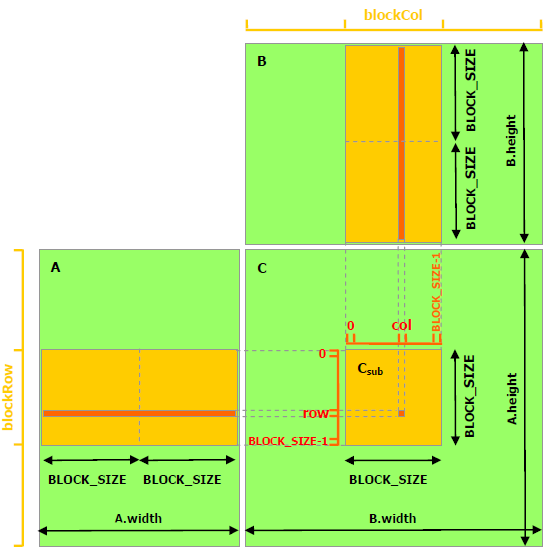
\includegraphics[width=0.8\textwidth, keepaspectratio]{images/ch02/CUDA-matrix-multiplication-by-blocks-using-shared-memory.png}
	\caption{Visualization of matrix multiplication by blocks of elements using shared memory.
		Note that this figure, taken from \citetitle{NVIDIADecember2022} \cite{NVIDIADecember2022}, depicts regular matrix multiplication, i.e., not the limited rendition present in Crout's method.
		The implementation in Listing~\ref{Listing:implementation->decomposition-project->implemented-solutions->decomposers->ICMxPP->kernels->diagonal-compute} performs matrix multiplication until the element that is being computed in terms of LU decomposition, as shown in Figure~\ref{Figure:theory->ICMPP->LUP->CMPP->sum-in-element-computation-dependance} on Page~\pageref{Figure:theory->ICMPP->LUP->CMPP->sum-in-element-computation-dependance}.
	}
	\label{Figure:implementation->decomposition-project->implemented-solutions->decomposers->ICMxPP->CUDA-matrix-multiplication-with-shared-memory}
\end{figure}

At the end of the kernel shown in Listing~\ref{Listing:implementation->decomposition-project->implemented-solutions->decomposers->ICMxPP->kernels->diagonal-compute}, it can be seen that the computed value, stored in the \code{sum} local variable, is saved into \code{LUnext} rather than \code{LU}.
This is done on purpose to avoid inconsistent results as threads would otherwise be able to overwrite values before other threads would be able to use them to compute their elements.
While it can be argued that this behavior may lead to higher performance due to fewer iterations being required, it is not stable and therefore a correct result cannot be guaranteed.
Thus, the assignment of values to \code{LU} for the next iteration takes place in the \code{DSecAssign\_kernel()} which is executed after the \code{DSecCompute\_kernel()}.
The \code{DSecAssign\_kernel()} kernel is shown in Listing~\ref{Listing:implementation->decomposition-project->implemented-solutions->decomposers->ICMxPP->kernels->diagonal-assign}.

\begin{lstlisting}[caption={The implementation of the \code{DSecAssign\_kernel()} kernel that assigns values of the next iteration to the matrix representing the current iteration.
Note that the matrices are passed using their views and the indices are copied to the local memory of each thread.},label={Listing:implementation->decomposition-project->implemented-solutions->decomposers->ICMxPP->kernels->diagonal-assign},escapechar=@]
template< typename MatrixView, typename Index >
__global__
void
DSecAssign_kernel( MatrixView LU, MatrixView LUnext, const Index sec_start_col, const Index sec_end_col, const Index sec_start_row, const Index sec_end_row, const Index badEl_rowcol )
{
	// Each thread computes one element (row, col)
	Index row = blockIdx.y * blockDim.y + threadIdx.y + sec_start_row;
	Index col = blockIdx.x * blockDim.x + threadIdx.x + sec_start_col;
	
	// Terminate threads that overreach the bounds
	if( row >= sec_end_row || col >= sec_end_col )
		return;
	
	// Terminate threads that would write elements to the bottom-right of the bad element
	if( row >= badEl_rowcol && col > badEl_rowcol ) @\label{Line:implementation->decomposition-project->implemented-solutions->decomposers->ICMxPP->kernels->diagonal-assign->terminate-threads-writing-past-badEl}@
		return;
	
	// Assign the values of the next iteration to the matrix representing the current iteration
	LU( row, col ) = LUnext( row, col );
}
\end{lstlisting}

It is noteworthy that the values located to the bottom-right of the bad element are excluded from the assignment.
The reasoning behind this is that those values are not computed by the preceding kernel as they would not be high-quality.
Therefore, their assignment is omitted to mitigate unnecessary accesses to global memory.

The kernels for computing the lower and right sections are similar to that of the diagonal section, therefore, they are included in Listings~\ref{Listing:ICMxPP-implementation->kernels->lower-section-compute} and \ref{Listing:ICMxPP-implementation->kernels->right-section-compute}, respectively.
Similarly, the assignment kernel for non-diagonal sections is shown only in Listing~\ref{Listing:ICMxPP-implementation->kernels->nondiagonal-assign}.

\subsubsection{Solvers}\label{Subsection:implementation->decomposition-project->implemented-solutions->solvers}
The \textit{Solvers} group consists of implementations that, given the output of an LU decomposition algorithm, solve a linear system.
To solve a linear system, solvers perform the operations described in Step~\ref{Item:theory->ICMPP->LUP->solving-system-linear-equations->substitution} of the two-step process mentioned in Section~\ref{Subsection:theory->ICMPP->LUP}.
For convenience, the operations are summarized below.

Specifically, assuming a system of $n \in \mathbb{N}$ linear equations with $n$ unknowns and $m \in \mathbb{N}$ right-hand sides, solvers solve a linear system defined as $\mathbf{LUX} = \mathbf{PB}$, where $\mathbf{L}$ and $\mathbf{U}$ are the output of an LU decomposition algorithm, $\mathbf{X}$ is an $n$-by-$m$ matrix of unknowns, $\mathbf{P}$ is an $n$-by-$n$ permutation matrix, and $\mathbf{B}$ is an $n$-by-$m$ matrix of right-hand sides.
In the context of the Decomposition project, solvers perform the following steps:

\begin{enumerate}
	\item If partial pivoting is enabled, permute the rows of matrix $\mathbf{B}$ according to matrix $\mathbf{P}$.
	\item \label{Item:implementation->decomposition-project->implemented-solutions->solvers->forward-substitution}
		Perform forward substitution by solving $\mathbf{LY} = \mathbf{B}$.
	\item \label{Item:implementation->decomposition-project->implemented-solutions->solvers->backward-substitution}
		Perform backward substitution by solving $\mathbf{UX} = \mathbf{Y}$.
\end{enumerate}

At the end of Step~\ref{Item:implementation->decomposition-project->implemented-solutions->solvers->backward-substitution} matrix $\mathbf{X}$ contains the values of the unknowns in the correct order.
In other words, $\mathbf{X}$ can be directly applied to $\mathbf{AX} = \mathbf{B}$ without the need for permutation.

The full list of solvers and their characteristics is presented in Table~\ref{Table:implementation->decomposition-project->implemented-solutions->solvers->solvers-in-the-project}.

\begin{table}[!ht]
	\centering
	\begin{tabular}{|l|l|l|l|}
		\hline
		\rowcolor[HTML]{C0C0C0}\textbf{Solver}              & \textbf{With / Without PP} & \textbf{Unit diag. in}     & \textbf{Device supported} \\ \hline
		\cellcolor[HTML]{EFEFEF}\textbf{SS(PP)}             & Yes / Yes                  & $\mathbf{U}$               & CPU                       \\
		\cellcolor[HTML]{EFEFEF}CuBLAStrsm(PP)              & Yes / Yes                  & $\mathbf{L}$, $\mathbf{U}$ & GPU                       \\
		\cellcolor[HTML]{EFEFEF}CuSolverDnXgetrs(PP)        & Yes / Yes                  & $\mathbf{L}$               & GPU                       \\
		\cellcolor[HTML]{EFEFEF}\textbf{IS\_\textit{x}(PP)} & Yes / Yes                  & $\mathbf{U}$               & CPU, GPU                  \\ \hline
	\end{tabular}
	\caption{The solvers made available by the Decomposition project.
		The solvers in \textbf{bold} font were implemented by the author of the project.
		The "PP" suffix indicates whether partial pivoting is used.
		The "\textit{x}" in the name of certain solvers signifies their CUDA thread configuration.
		The "Unit diag. In" column indicates the format of the input matrix the solver supports, i.e., if the unit diagonal should be in $\mathbf{L}$, $\mathbf{U}$, or either.
	}
	\label{Table:implementation->decomposition-project->implemented-solutions->solvers->solvers-in-the-project}
\end{table}

As can be seen from Table~\ref{Table:implementation->decomposition-project->implemented-solutions->solvers->solvers-in-the-project}, two solvers were implemented as part of this project: SSPP and IS\_\textit{x}PP.

\paragraph{Sequential Solver with Partial Pivoting (SSPP)}\label{Paragraph:implementation->decomposition-project->implemented-solutions->solvers->SSPP}
Similarly to the CMPP decomposer, the Sequential Solver with partial pivoting (SSPP) is a basic algorithm implemented only for the CPU as its sequential algorithm would be inefficient on the GPU.

The purpose of the SSPP solver is to provide an accurate and simple solver.
Therefore, it was not optimized or improved upon except for adding support for multiple right-hand sides.
The definition of the \code{solve()} method for the SSPP solver is shown in Listing~\ref{Listing:SSPP-implementation-excerpt} of Appendix~\ref{Appendix:SSPP-implementation}.
The implementation showcases how multiple right-hand sides can be handled in forward substitution using \code{TNL::Algorithms::parallelFor()} (described in Section~\ref{Subsection:implementation->libraries-used->TNL->parallel-functionalities}).

\paragraph{Iterative Solver with Partial Pivoting (IS\_\textit{x}PP)}\label{Paragraph:implementation->decomposition-project->implemented-solutions->solvers->ISxPP}
The IS\_\textit{x}PP solver was implemented as an experimental method that aimed to combine the approach of ICM\_\textit{x}PP and the algorithm of SSPP.
However, it was not a part of the diploma thesis assignment and was therefore not prioritized in terms of optimization.
Thus, the implementation of IS\_\textit{x}PP is naive in the sense that it performs iterations of both substitutions until their respective matrices are processed.
In other words, it repeatedly computes all values in $\mathbf{LY} = \mathbf{B}$ simultaneously until the values of $\mathbf{Y}$ stop changing between iterations according to a set tolerance.
Then, it performs the same for $\mathbf{UX} = \mathbf{Y}$ and $\mathbf{X}$.
While the solver is implemented both for the CPU and the GPU, the former implementation serves solely as a means to verify the approach, therefore, it is not presented in this thesis.
The definition of the \code{solve()} method for the IS\_\textit{x}PP solver is shown in Listing~\ref{Listing:ISxPP-implementation-excerpt}.

\paragraph{Compatibility of Decomposers and Solvers} Combining the information from Tables~\ref{Table:implementation->decomposition-project->implemented-solutions->decomposers->decomposers-in-the-project} and \ref{Table:implementation->decomposition-project->implemented-solutions->solvers->solvers-in-the-project} yields the overview of compatible decomposers and solvers presented in Table~\ref{Table:implementation->decomposition-project->implemented-solutions->solvers->compatibile-decomposers-and-solvers}.

\begin{table}[!ht]
	\centering
	\begin{tabular}{|l|c|c|c|c|}
		\hline
		\rowcolor[HTML]{C0C0C0} \textbf{Decomposer} \textbackslash\space \textbf{Solver} & \cellcolor[HTML]{EFEFEF}SS(PP) & \cellcolor[HTML]{EFEFEF}IS\_\textit{x}(PP) & \cellcolor[HTML]{EFEFEF}CuBLAStrsm(PP) & \cellcolor[HTML]{EFEFEF}CuSolverDnXgetrs(PP) \\ \hline
		\cellcolor[HTML]{EFEFEF}CM(PP)               & Yes & Yes & Yes & No  \\
		\cellcolor[HTML]{EFEFEF}CuSolverDnXgetrf(PP) & No  & No  & Yes & Yes \\
		\cellcolor[HTML]{EFEFEF}ICM\_\textit{x}(PP)  & Yes & Yes & Yes & No  \\
		\cellcolor[HTML]{EFEFEF}PCM\_\textit{x}(PP)  & Yes & Yes & Yes & No  \\ \hline
	\end{tabular}
	\caption{Compatibility of decomposer and solvers made available by the Decomposition project.
		To clarify, a decomposer-solver combination is compatible if the two can be used to complete a linear solver.
	}
	\label{Table:implementation->decomposition-project->implemented-solutions->solvers->compatibile-decomposers-and-solvers}
\end{table}



\subsection{Benchmarks}\label{Subsection:implementation->decomposition-project->benchmarks}
One of the tasks for this thesis was to compare the performance of decomposers and solvers that were implemented by the author with that of established libraries.
For this purpose, a benchmark system was implemented for both decomposers and solvers.
It is important to note that while the benchmark system was implemented as part of \citetitle{Cejka2022} \cite{Cejka2022}, it was adapted from the SpMV TNL Benchmark structure\footnote{TNL SpMV Benchmark GitLab repository URL: \url{https://gitlab.com/tnl-project/tnl/-/tree/main/src/Benchmarks/SpMV}}.
However, with the introduction of partial pivoting into the project, the implementation underwent major refactoring.

This section briefly introduces the benchmark procedure for both decomposers and solvers.
First, steps that are common for both benchmarks are described.
Then, aspects specific to each benchmark are mentioned separately.

Both benchmarks are initiated via a Bash script that sets up the logging directory, compiles the benchmarks, and finally, launches the benchmark for each matrix found in a set directory.
Note that the benchmark is launched twice: first using double precision, then using single precision.
Each execution of the benchmark for a given matrix consists of the following steps:

\begin{enumerate}
	\item Load the matrix from its \code{.mtx} file.
The \code{mtx} file format is referred to as the \textit{Matrix Market File Format}\footnote{Matrix Market Exchange Formats URL: \url{https://math.nist.gov/MatrixMarket/formats.html\#MMformat}} and it is primarily used to represent sparse matrices as only nonzero entries are stored along with their coordinates.
	\item \label{Item:implementation->decomposition-project->benchmarks->procedure->baseline-operation}
		Perform the benchmarked operation using a baseline implementation, for example, CMPP.
	\item \label{Item:implementation->decomposition-project->benchmarks->procedure->selected-operations}
		Perform the benchmarked operation using a selected implementation.
\end{enumerate}

Each benchmarked operation can be performed in loops with the results of all loops averaged to amount for statistically significant results.
The results can include, for example, the execution time of the operation and its standard deviation, the maximum absolute difference between the actual results and the expected results, etc.
The averaged results are logged using \code{TNL::Benchmarks::JsonLogging} as JSON objects into log files which can be later transformed into HTML tables and MATLAB plots using a Python script provided in \code{src/Benchmarks/utils}.

Note that the maximum absolute difference is computed on the CPU to assure the highest possible accuracy.
The maximum absolute difference is defined for decomposers as:

\begin{equation}
	\max \left| \mathbf{A} - \mathbf{PLU} \right| \,,
	\label{Equation:implementation->decomposition-project->benchmarks->decomposers->maximum-difference}
\end{equation}

where $\mathbf{A}$ is the input matrix, $\mathbf{P}$ is the permutation matrix (represented in code by a pivoting vector), and matrices $\mathbf{L}$ and $\mathbf{U}$ are the results of the LU decomposition operation.
To clarify, the maximum absolute difference for decomposers is the largest absolute difference between a computed element and its expected result.

For solvers the maximum absolute difference is defined as:

\begin{equation}
	\max \left| \mathbf{PLUX} - \mathbf{B} \right| \,,
	\label{Equation:implementation->decomposition-project->benchmarks->solvers->maximum-difference}
\end{equation}

where matrices $\mathbf{P}$, $\mathbf{L}$, and $\mathbf{U}$ are the same as in Equation~\ref{Equation:implementation->decomposition-project->benchmarks->decomposers->maximum-difference}, $\mathbf{X}$ is the computed matrix of unknowns, and $\mathbf{B}$ is the matrix of right-hand sides.
To clarify, the computed unknowns are used in the system of equations in matrix form, and then the largest absolute difference between the left- and right-hand sides is used.

As mentioned in \citetitle{Cejka2022} \cite{Cejka2022}, many aspects of the implementations can only be verified on larger matrices.
Thus, aside from unit tests, benchmarks were a crucial part of assuring the quality of the implementations.




\section{BDDCML Integration}\label{Section:implementation->BDDCML}
Another key task for this thesis was to apply the decomposers and solvers made available by the Decomposition project in the Multilevel BDDC Solver Library (BDDCML) \cite{Sistek2011, Sistek2012, Sousedik2013, Sistek2015}.
According to the project's website\footnote{\label{Footnote:implementation->BDDCML-integration->BDDCML-website}BDDCML website URL: \url{https://users.math.cas.cz/~sistek/software/bddcml.html}}, the goal of BDDCML is to provide a scalable parallel solver of linear equations for systems originating from finite element computations.
The implementation of the library was inspired by the Adaptive-Multilevel variant of the Balancing Domain Decomposition by Constraints (BDDC) method.
More information regarding BDDCML can be found on its website\footref{Footnote:implementation->BDDCML-integration->BDDCML-website} or in its GitHub repository\footnote{Multilevel BDDC Solver Library GitHub repository URL: \url{https://github.com/sistek/bddcml}}.

\paragraph{Integration with the Decomposition Project} BDDCML is written in Fortran 95 and the Decomposition project is written in C++.
Therefore, to use decomposers and solvers from the Decomposition project in BDDCML, the TNL-BDDCML Interface\footnote{tnl\_bddcml\_interface Bitbucket repository URL: \url{https://bitbucket.org/tnl-decomposition/tnl_bddcml_interface/src/master}} was used.
The interface was implemented by Ing.
Jakub Šístek, Ph.D. as a means to use data structures and functionalities provided by TNL in BDDCML, for example, the allocation and deallocation of a \code{TNL::Matrices::DenseMatrix} instance on the GPU, GEMV, etc.\\
For the Decomposition project, Fortran wrappers calling the \code{decompose()} method of a specific decomposer or the \code{solve()} method of a specific solver were added to the interface.

Note that both the interface and BDDCML needed to be extended.
Therefore, the repositories were forked and the changes related to the Decomposition project were added separately.
The final versions of both repositories that contain changes related to the Decomposition project are available on request or as an attachment to this thesis.

\paragraph{Benchmarks} The performance of decomposers and solvers provided by the Decomposition project is compared with the corresponding routines of the MAGMA library \cite{Tomov2010} which was already used in BDDCML.
In particular, the performance was compared when solving the "Poisson equation on a cube" problem present in BDDCML.
Furthermore, for the results of the performance comparison to be statistically significant, a benchmarking system was implemented.
The system comprises:

\begin{tight_itemize}
	\item \code{prepare\_poisson\_on\_cube\_benchmark} - The Bash script that compiles BDDCML with different combinations of decomposers and solvers.
	\item \code{run\_poisson\_on\_cube\_benchmark} - The Bash script that runs the \code{poisson\_on\_cube} executable in loops and sorts logs into directories.
	\item \code{poisson\_on\_cube\_logs\_to\_csv.py} - The Python script that parses the logs for results, for example, total time taken by a procedure, total time of execution, the accuracy of the solution, etc.
These results, obtained across several loops, are then averaged and saved into a CSV file and plotted using MATLAB.
\end{tight_itemize}